\documentclass[11pt]{article}

    \usepackage[breakable]{tcolorbox}
    \usepackage{parskip} % Stop auto-indenting (to mimic markdown behaviour)
    
    \usepackage{iftex}
    \ifPDFTeX
    	\usepackage[T1]{fontenc}
    	\usepackage{mathpazo}
    \else
    	\usepackage{fontspec}
    \fi

    % Basic figure setup, for now with no caption control since it's done
    % automatically by Pandoc (which extracts ![](path) syntax from Markdown).
    \usepackage{graphicx}
    % Maintain compatibility with old templates. Remove in nbconvert 6.0
    \let\Oldincludegraphics\includegraphics
    % Ensure that by default, figures have no caption (until we provide a
    % proper Figure object with a Caption API and a way to capture that
    % in the conversion process - todo).
    \usepackage{caption}
    \DeclareCaptionFormat{nocaption}{}
    \captionsetup{format=nocaption,aboveskip=0pt,belowskip=0pt}

    \usepackage{float}
    \floatplacement{figure}{H} % forces figures to be placed at the correct location
    \usepackage{xcolor} % Allow colors to be defined
    \usepackage{enumerate} % Needed for markdown enumerations to work
    \usepackage{geometry} % Used to adjust the document margins
    \usepackage{amsmath} % Equations
    \usepackage{amssymb} % Equations
    \usepackage{textcomp} % defines textquotesingle
    % Hack from http://tex.stackexchange.com/a/47451/13684:
    \AtBeginDocument{%
        \def\PYZsq{\textquotesingle}% Upright quotes in Pygmentized code
    }
    \usepackage{upquote} % Upright quotes for verbatim code
    \usepackage{eurosym} % defines \euro
    \usepackage[mathletters]{ucs} % Extended unicode (utf-8) support
    \usepackage{fancyvrb} % verbatim replacement that allows latex
    \usepackage{grffile} % extends the file name processing of package graphics 
                         % to support a larger range
    \makeatletter % fix for old versions of grffile with XeLaTeX
    \@ifpackagelater{grffile}{2019/11/01}
    {
      % Do nothing on new versions
    }
    {
      \def\Gread@@xetex#1{%
        \IfFileExists{"\Gin@base".bb}%
        {\Gread@eps{\Gin@base.bb}}%
        {\Gread@@xetex@aux#1}%
      }
    }
    \makeatother
    \usepackage[Export]{adjustbox} % Used to constrain images to a maximum size
    \adjustboxset{max size={0.9\linewidth}{0.9\paperheight}}

    % The hyperref package gives us a pdf with properly built
    % internal navigation ('pdf bookmarks' for the table of contents,
    % internal cross-reference links, web links for URLs, etc.)
    \usepackage{hyperref}
    % The default LaTeX title has an obnoxious amount of whitespace. By default,
    % titling removes some of it. It also provides customization options.
    \usepackage{titling}
    \usepackage{longtable} % longtable support required by pandoc >1.10
    \usepackage{booktabs}  % table support for pandoc > 1.12.2
    \usepackage[inline]{enumitem} % IRkernel/repr support (it uses the enumerate* environment)
    \usepackage[normalem]{ulem} % ulem is needed to support strikethroughs (\sout)
                                % normalem makes italics be italics, not underlines
    \usepackage{mathrsfs}
    

    
    % Colors for the hyperref package
    \definecolor{urlcolor}{rgb}{0,.145,.698}
    \definecolor{linkcolor}{rgb}{.71,0.21,0.01}
    \definecolor{citecolor}{rgb}{.12,.54,.11}

    % ANSI colors
    \definecolor{ansi-black}{HTML}{3E424D}
    \definecolor{ansi-black-intense}{HTML}{282C36}
    \definecolor{ansi-red}{HTML}{E75C58}
    \definecolor{ansi-red-intense}{HTML}{B22B31}
    \definecolor{ansi-green}{HTML}{00A250}
    \definecolor{ansi-green-intense}{HTML}{007427}
    \definecolor{ansi-yellow}{HTML}{DDB62B}
    \definecolor{ansi-yellow-intense}{HTML}{B27D12}
    \definecolor{ansi-blue}{HTML}{208FFB}
    \definecolor{ansi-blue-intense}{HTML}{0065CA}
    \definecolor{ansi-magenta}{HTML}{D160C4}
    \definecolor{ansi-magenta-intense}{HTML}{A03196}
    \definecolor{ansi-cyan}{HTML}{60C6C8}
    \definecolor{ansi-cyan-intense}{HTML}{258F8F}
    \definecolor{ansi-white}{HTML}{C5C1B4}
    \definecolor{ansi-white-intense}{HTML}{A1A6B2}
    \definecolor{ansi-default-inverse-fg}{HTML}{FFFFFF}
    \definecolor{ansi-default-inverse-bg}{HTML}{000000}

    % common color for the border for error outputs.
    \definecolor{outerrorbackground}{HTML}{FFDFDF}

    % commands and environments needed by pandoc snippets
    % extracted from the output of `pandoc -s`
    \providecommand{\tightlist}{%
      \setlength{\itemsep}{0pt}\setlength{\parskip}{0pt}}
    \DefineVerbatimEnvironment{Highlighting}{Verbatim}{commandchars=\\\{\}}
    % Add ',fontsize=\small' for more characters per line
    \newenvironment{Shaded}{}{}
    \newcommand{\KeywordTok}[1]{\textcolor[rgb]{0.00,0.44,0.13}{\textbf{{#1}}}}
    \newcommand{\DataTypeTok}[1]{\textcolor[rgb]{0.56,0.13,0.00}{{#1}}}
    \newcommand{\DecValTok}[1]{\textcolor[rgb]{0.25,0.63,0.44}{{#1}}}
    \newcommand{\BaseNTok}[1]{\textcolor[rgb]{0.25,0.63,0.44}{{#1}}}
    \newcommand{\FloatTok}[1]{\textcolor[rgb]{0.25,0.63,0.44}{{#1}}}
    \newcommand{\CharTok}[1]{\textcolor[rgb]{0.25,0.44,0.63}{{#1}}}
    \newcommand{\StringTok}[1]{\textcolor[rgb]{0.25,0.44,0.63}{{#1}}}
    \newcommand{\CommentTok}[1]{\textcolor[rgb]{0.38,0.63,0.69}{\textit{{#1}}}}
    \newcommand{\OtherTok}[1]{\textcolor[rgb]{0.00,0.44,0.13}{{#1}}}
    \newcommand{\AlertTok}[1]{\textcolor[rgb]{1.00,0.00,0.00}{\textbf{{#1}}}}
    \newcommand{\FunctionTok}[1]{\textcolor[rgb]{0.02,0.16,0.49}{{#1}}}
    \newcommand{\RegionMarkerTok}[1]{{#1}}
    \newcommand{\ErrorTok}[1]{\textcolor[rgb]{1.00,0.00,0.00}{\textbf{{#1}}}}
    \newcommand{\NormalTok}[1]{{#1}}
    
    % Additional commands for more recent versions of Pandoc
    \newcommand{\ConstantTok}[1]{\textcolor[rgb]{0.53,0.00,0.00}{{#1}}}
    \newcommand{\SpecialCharTok}[1]{\textcolor[rgb]{0.25,0.44,0.63}{{#1}}}
    \newcommand{\VerbatimStringTok}[1]{\textcolor[rgb]{0.25,0.44,0.63}{{#1}}}
    \newcommand{\SpecialStringTok}[1]{\textcolor[rgb]{0.73,0.40,0.53}{{#1}}}
    \newcommand{\ImportTok}[1]{{#1}}
    \newcommand{\DocumentationTok}[1]{\textcolor[rgb]{0.73,0.13,0.13}{\textit{{#1}}}}
    \newcommand{\AnnotationTok}[1]{\textcolor[rgb]{0.38,0.63,0.69}{\textbf{\textit{{#1}}}}}
    \newcommand{\CommentVarTok}[1]{\textcolor[rgb]{0.38,0.63,0.69}{\textbf{\textit{{#1}}}}}
    \newcommand{\VariableTok}[1]{\textcolor[rgb]{0.10,0.09,0.49}{{#1}}}
    \newcommand{\ControlFlowTok}[1]{\textcolor[rgb]{0.00,0.44,0.13}{\textbf{{#1}}}}
    \newcommand{\OperatorTok}[1]{\textcolor[rgb]{0.40,0.40,0.40}{{#1}}}
    \newcommand{\BuiltInTok}[1]{{#1}}
    \newcommand{\ExtensionTok}[1]{{#1}}
    \newcommand{\PreprocessorTok}[1]{\textcolor[rgb]{0.74,0.48,0.00}{{#1}}}
    \newcommand{\AttributeTok}[1]{\textcolor[rgb]{0.49,0.56,0.16}{{#1}}}
    \newcommand{\InformationTok}[1]{\textcolor[rgb]{0.38,0.63,0.69}{\textbf{\textit{{#1}}}}}
    \newcommand{\WarningTok}[1]{\textcolor[rgb]{0.38,0.63,0.69}{\textbf{\textit{{#1}}}}}
    
    
    % Define a nice break command that doesn't care if a line doesn't already
    % exist.
    \def\br{\hspace*{\fill} \\* }
    % Math Jax compatibility definitions
    \def\gt{>}
    \def\lt{<}
    \let\Oldtex\TeX
    \let\Oldlatex\LaTeX
    \renewcommand{\TeX}{\textrm{\Oldtex}}
    \renewcommand{\LaTeX}{\textrm{\Oldlatex}}
    % Document parameters
    % Document title
    \title{GreatBasin}
    
    
    
    
    
% Pygments definitions
\makeatletter
\def\PY@reset{\let\PY@it=\relax \let\PY@bf=\relax%
    \let\PY@ul=\relax \let\PY@tc=\relax%
    \let\PY@bc=\relax \let\PY@ff=\relax}
\def\PY@tok#1{\csname PY@tok@#1\endcsname}
\def\PY@toks#1+{\ifx\relax#1\empty\else%
    \PY@tok{#1}\expandafter\PY@toks\fi}
\def\PY@do#1{\PY@bc{\PY@tc{\PY@ul{%
    \PY@it{\PY@bf{\PY@ff{#1}}}}}}}
\def\PY#1#2{\PY@reset\PY@toks#1+\relax+\PY@do{#2}}

\@namedef{PY@tok@w}{\def\PY@tc##1{\textcolor[rgb]{0.73,0.73,0.73}{##1}}}
\@namedef{PY@tok@c}{\let\PY@it=\textit\def\PY@tc##1{\textcolor[rgb]{0.25,0.50,0.50}{##1}}}
\@namedef{PY@tok@cp}{\def\PY@tc##1{\textcolor[rgb]{0.74,0.48,0.00}{##1}}}
\@namedef{PY@tok@k}{\let\PY@bf=\textbf\def\PY@tc##1{\textcolor[rgb]{0.00,0.50,0.00}{##1}}}
\@namedef{PY@tok@kp}{\def\PY@tc##1{\textcolor[rgb]{0.00,0.50,0.00}{##1}}}
\@namedef{PY@tok@kt}{\def\PY@tc##1{\textcolor[rgb]{0.69,0.00,0.25}{##1}}}
\@namedef{PY@tok@o}{\def\PY@tc##1{\textcolor[rgb]{0.40,0.40,0.40}{##1}}}
\@namedef{PY@tok@ow}{\let\PY@bf=\textbf\def\PY@tc##1{\textcolor[rgb]{0.67,0.13,1.00}{##1}}}
\@namedef{PY@tok@nb}{\def\PY@tc##1{\textcolor[rgb]{0.00,0.50,0.00}{##1}}}
\@namedef{PY@tok@nf}{\def\PY@tc##1{\textcolor[rgb]{0.00,0.00,1.00}{##1}}}
\@namedef{PY@tok@nc}{\let\PY@bf=\textbf\def\PY@tc##1{\textcolor[rgb]{0.00,0.00,1.00}{##1}}}
\@namedef{PY@tok@nn}{\let\PY@bf=\textbf\def\PY@tc##1{\textcolor[rgb]{0.00,0.00,1.00}{##1}}}
\@namedef{PY@tok@ne}{\let\PY@bf=\textbf\def\PY@tc##1{\textcolor[rgb]{0.82,0.25,0.23}{##1}}}
\@namedef{PY@tok@nv}{\def\PY@tc##1{\textcolor[rgb]{0.10,0.09,0.49}{##1}}}
\@namedef{PY@tok@no}{\def\PY@tc##1{\textcolor[rgb]{0.53,0.00,0.00}{##1}}}
\@namedef{PY@tok@nl}{\def\PY@tc##1{\textcolor[rgb]{0.63,0.63,0.00}{##1}}}
\@namedef{PY@tok@ni}{\let\PY@bf=\textbf\def\PY@tc##1{\textcolor[rgb]{0.60,0.60,0.60}{##1}}}
\@namedef{PY@tok@na}{\def\PY@tc##1{\textcolor[rgb]{0.49,0.56,0.16}{##1}}}
\@namedef{PY@tok@nt}{\let\PY@bf=\textbf\def\PY@tc##1{\textcolor[rgb]{0.00,0.50,0.00}{##1}}}
\@namedef{PY@tok@nd}{\def\PY@tc##1{\textcolor[rgb]{0.67,0.13,1.00}{##1}}}
\@namedef{PY@tok@s}{\def\PY@tc##1{\textcolor[rgb]{0.73,0.13,0.13}{##1}}}
\@namedef{PY@tok@sd}{\let\PY@it=\textit\def\PY@tc##1{\textcolor[rgb]{0.73,0.13,0.13}{##1}}}
\@namedef{PY@tok@si}{\let\PY@bf=\textbf\def\PY@tc##1{\textcolor[rgb]{0.73,0.40,0.53}{##1}}}
\@namedef{PY@tok@se}{\let\PY@bf=\textbf\def\PY@tc##1{\textcolor[rgb]{0.73,0.40,0.13}{##1}}}
\@namedef{PY@tok@sr}{\def\PY@tc##1{\textcolor[rgb]{0.73,0.40,0.53}{##1}}}
\@namedef{PY@tok@ss}{\def\PY@tc##1{\textcolor[rgb]{0.10,0.09,0.49}{##1}}}
\@namedef{PY@tok@sx}{\def\PY@tc##1{\textcolor[rgb]{0.00,0.50,0.00}{##1}}}
\@namedef{PY@tok@m}{\def\PY@tc##1{\textcolor[rgb]{0.40,0.40,0.40}{##1}}}
\@namedef{PY@tok@gh}{\let\PY@bf=\textbf\def\PY@tc##1{\textcolor[rgb]{0.00,0.00,0.50}{##1}}}
\@namedef{PY@tok@gu}{\let\PY@bf=\textbf\def\PY@tc##1{\textcolor[rgb]{0.50,0.00,0.50}{##1}}}
\@namedef{PY@tok@gd}{\def\PY@tc##1{\textcolor[rgb]{0.63,0.00,0.00}{##1}}}
\@namedef{PY@tok@gi}{\def\PY@tc##1{\textcolor[rgb]{0.00,0.63,0.00}{##1}}}
\@namedef{PY@tok@gr}{\def\PY@tc##1{\textcolor[rgb]{1.00,0.00,0.00}{##1}}}
\@namedef{PY@tok@ge}{\let\PY@it=\textit}
\@namedef{PY@tok@gs}{\let\PY@bf=\textbf}
\@namedef{PY@tok@gp}{\let\PY@bf=\textbf\def\PY@tc##1{\textcolor[rgb]{0.00,0.00,0.50}{##1}}}
\@namedef{PY@tok@go}{\def\PY@tc##1{\textcolor[rgb]{0.53,0.53,0.53}{##1}}}
\@namedef{PY@tok@gt}{\def\PY@tc##1{\textcolor[rgb]{0.00,0.27,0.87}{##1}}}
\@namedef{PY@tok@err}{\def\PY@bc##1{{\setlength{\fboxsep}{-\fboxrule}\fcolorbox[rgb]{1.00,0.00,0.00}{1,1,1}{\strut ##1}}}}
\@namedef{PY@tok@kc}{\let\PY@bf=\textbf\def\PY@tc##1{\textcolor[rgb]{0.00,0.50,0.00}{##1}}}
\@namedef{PY@tok@kd}{\let\PY@bf=\textbf\def\PY@tc##1{\textcolor[rgb]{0.00,0.50,0.00}{##1}}}
\@namedef{PY@tok@kn}{\let\PY@bf=\textbf\def\PY@tc##1{\textcolor[rgb]{0.00,0.50,0.00}{##1}}}
\@namedef{PY@tok@kr}{\let\PY@bf=\textbf\def\PY@tc##1{\textcolor[rgb]{0.00,0.50,0.00}{##1}}}
\@namedef{PY@tok@bp}{\def\PY@tc##1{\textcolor[rgb]{0.00,0.50,0.00}{##1}}}
\@namedef{PY@tok@fm}{\def\PY@tc##1{\textcolor[rgb]{0.00,0.00,1.00}{##1}}}
\@namedef{PY@tok@vc}{\def\PY@tc##1{\textcolor[rgb]{0.10,0.09,0.49}{##1}}}
\@namedef{PY@tok@vg}{\def\PY@tc##1{\textcolor[rgb]{0.10,0.09,0.49}{##1}}}
\@namedef{PY@tok@vi}{\def\PY@tc##1{\textcolor[rgb]{0.10,0.09,0.49}{##1}}}
\@namedef{PY@tok@vm}{\def\PY@tc##1{\textcolor[rgb]{0.10,0.09,0.49}{##1}}}
\@namedef{PY@tok@sa}{\def\PY@tc##1{\textcolor[rgb]{0.73,0.13,0.13}{##1}}}
\@namedef{PY@tok@sb}{\def\PY@tc##1{\textcolor[rgb]{0.73,0.13,0.13}{##1}}}
\@namedef{PY@tok@sc}{\def\PY@tc##1{\textcolor[rgb]{0.73,0.13,0.13}{##1}}}
\@namedef{PY@tok@dl}{\def\PY@tc##1{\textcolor[rgb]{0.73,0.13,0.13}{##1}}}
\@namedef{PY@tok@s2}{\def\PY@tc##1{\textcolor[rgb]{0.73,0.13,0.13}{##1}}}
\@namedef{PY@tok@sh}{\def\PY@tc##1{\textcolor[rgb]{0.73,0.13,0.13}{##1}}}
\@namedef{PY@tok@s1}{\def\PY@tc##1{\textcolor[rgb]{0.73,0.13,0.13}{##1}}}
\@namedef{PY@tok@mb}{\def\PY@tc##1{\textcolor[rgb]{0.40,0.40,0.40}{##1}}}
\@namedef{PY@tok@mf}{\def\PY@tc##1{\textcolor[rgb]{0.40,0.40,0.40}{##1}}}
\@namedef{PY@tok@mh}{\def\PY@tc##1{\textcolor[rgb]{0.40,0.40,0.40}{##1}}}
\@namedef{PY@tok@mi}{\def\PY@tc##1{\textcolor[rgb]{0.40,0.40,0.40}{##1}}}
\@namedef{PY@tok@il}{\def\PY@tc##1{\textcolor[rgb]{0.40,0.40,0.40}{##1}}}
\@namedef{PY@tok@mo}{\def\PY@tc##1{\textcolor[rgb]{0.40,0.40,0.40}{##1}}}
\@namedef{PY@tok@ch}{\let\PY@it=\textit\def\PY@tc##1{\textcolor[rgb]{0.25,0.50,0.50}{##1}}}
\@namedef{PY@tok@cm}{\let\PY@it=\textit\def\PY@tc##1{\textcolor[rgb]{0.25,0.50,0.50}{##1}}}
\@namedef{PY@tok@cpf}{\let\PY@it=\textit\def\PY@tc##1{\textcolor[rgb]{0.25,0.50,0.50}{##1}}}
\@namedef{PY@tok@c1}{\let\PY@it=\textit\def\PY@tc##1{\textcolor[rgb]{0.25,0.50,0.50}{##1}}}
\@namedef{PY@tok@cs}{\let\PY@it=\textit\def\PY@tc##1{\textcolor[rgb]{0.25,0.50,0.50}{##1}}}

\def\PYZbs{\char`\\}
\def\PYZus{\char`\_}
\def\PYZob{\char`\{}
\def\PYZcb{\char`\}}
\def\PYZca{\char`\^}
\def\PYZam{\char`\&}
\def\PYZlt{\char`\<}
\def\PYZgt{\char`\>}
\def\PYZsh{\char`\#}
\def\PYZpc{\char`\%}
\def\PYZdl{\char`\$}
\def\PYZhy{\char`\-}
\def\PYZsq{\char`\'}
\def\PYZdq{\char`\"}
\def\PYZti{\char`\~}
% for compatibility with earlier versions
\def\PYZat{@}
\def\PYZlb{[}
\def\PYZrb{]}
\makeatother


    % For linebreaks inside Verbatim environment from package fancyvrb. 
    \makeatletter
        \newbox\Wrappedcontinuationbox 
        \newbox\Wrappedvisiblespacebox 
        \newcommand*\Wrappedvisiblespace {\textcolor{red}{\textvisiblespace}} 
        \newcommand*\Wrappedcontinuationsymbol {\textcolor{red}{\llap{\tiny$\m@th\hookrightarrow$}}} 
        \newcommand*\Wrappedcontinuationindent {3ex } 
        \newcommand*\Wrappedafterbreak {\kern\Wrappedcontinuationindent\copy\Wrappedcontinuationbox} 
        % Take advantage of the already applied Pygments mark-up to insert 
        % potential linebreaks for TeX processing. 
        %        {, <, #, %, $, ' and ": go to next line. 
        %        _, }, ^, &, >, - and ~: stay at end of broken line. 
        % Use of \textquotesingle for straight quote. 
        \newcommand*\Wrappedbreaksatspecials {% 
            \def\PYGZus{\discretionary{\char`\_}{\Wrappedafterbreak}{\char`\_}}% 
            \def\PYGZob{\discretionary{}{\Wrappedafterbreak\char`\{}{\char`\{}}% 
            \def\PYGZcb{\discretionary{\char`\}}{\Wrappedafterbreak}{\char`\}}}% 
            \def\PYGZca{\discretionary{\char`\^}{\Wrappedafterbreak}{\char`\^}}% 
            \def\PYGZam{\discretionary{\char`\&}{\Wrappedafterbreak}{\char`\&}}% 
            \def\PYGZlt{\discretionary{}{\Wrappedafterbreak\char`\<}{\char`\<}}% 
            \def\PYGZgt{\discretionary{\char`\>}{\Wrappedafterbreak}{\char`\>}}% 
            \def\PYGZsh{\discretionary{}{\Wrappedafterbreak\char`\#}{\char`\#}}% 
            \def\PYGZpc{\discretionary{}{\Wrappedafterbreak\char`\%}{\char`\%}}% 
            \def\PYGZdl{\discretionary{}{\Wrappedafterbreak\char`\$}{\char`\$}}% 
            \def\PYGZhy{\discretionary{\char`\-}{\Wrappedafterbreak}{\char`\-}}% 
            \def\PYGZsq{\discretionary{}{\Wrappedafterbreak\textquotesingle}{\textquotesingle}}% 
            \def\PYGZdq{\discretionary{}{\Wrappedafterbreak\char`\"}{\char`\"}}% 
            \def\PYGZti{\discretionary{\char`\~}{\Wrappedafterbreak}{\char`\~}}% 
        } 
        % Some characters . , ; ? ! / are not pygmentized. 
        % This macro makes them "active" and they will insert potential linebreaks 
        \newcommand*\Wrappedbreaksatpunct {% 
            \lccode`\~`\.\lowercase{\def~}{\discretionary{\hbox{\char`\.}}{\Wrappedafterbreak}{\hbox{\char`\.}}}% 
            \lccode`\~`\,\lowercase{\def~}{\discretionary{\hbox{\char`\,}}{\Wrappedafterbreak}{\hbox{\char`\,}}}% 
            \lccode`\~`\;\lowercase{\def~}{\discretionary{\hbox{\char`\;}}{\Wrappedafterbreak}{\hbox{\char`\;}}}% 
            \lccode`\~`\:\lowercase{\def~}{\discretionary{\hbox{\char`\:}}{\Wrappedafterbreak}{\hbox{\char`\:}}}% 
            \lccode`\~`\?\lowercase{\def~}{\discretionary{\hbox{\char`\?}}{\Wrappedafterbreak}{\hbox{\char`\?}}}% 
            \lccode`\~`\!\lowercase{\def~}{\discretionary{\hbox{\char`\!}}{\Wrappedafterbreak}{\hbox{\char`\!}}}% 
            \lccode`\~`\/\lowercase{\def~}{\discretionary{\hbox{\char`\/}}{\Wrappedafterbreak}{\hbox{\char`\/}}}% 
            \catcode`\.\active
            \catcode`\,\active 
            \catcode`\;\active
            \catcode`\:\active
            \catcode`\?\active
            \catcode`\!\active
            \catcode`\/\active 
            \lccode`\~`\~ 	
        }
    \makeatother

    \let\OriginalVerbatim=\Verbatim
    \makeatletter
    \renewcommand{\Verbatim}[1][1]{%
        %\parskip\z@skip
        \sbox\Wrappedcontinuationbox {\Wrappedcontinuationsymbol}%
        \sbox\Wrappedvisiblespacebox {\FV@SetupFont\Wrappedvisiblespace}%
        \def\FancyVerbFormatLine ##1{\hsize\linewidth
            \vtop{\raggedright\hyphenpenalty\z@\exhyphenpenalty\z@
                \doublehyphendemerits\z@\finalhyphendemerits\z@
                \strut ##1\strut}%
        }%
        % If the linebreak is at a space, the latter will be displayed as visible
        % space at end of first line, and a continuation symbol starts next line.
        % Stretch/shrink are however usually zero for typewriter font.
        \def\FV@Space {%
            \nobreak\hskip\z@ plus\fontdimen3\font minus\fontdimen4\font
            \discretionary{\copy\Wrappedvisiblespacebox}{\Wrappedafterbreak}
            {\kern\fontdimen2\font}%
        }%
        
        % Allow breaks at special characters using \PYG... macros.
        \Wrappedbreaksatspecials
        % Breaks at punctuation characters . , ; ? ! and / need catcode=\active 	
        \OriginalVerbatim[#1,codes*=\Wrappedbreaksatpunct]%
    }
    \makeatother

    % Exact colors from NB
    \definecolor{incolor}{HTML}{303F9F}
    \definecolor{outcolor}{HTML}{D84315}
    \definecolor{cellborder}{HTML}{CFCFCF}
    \definecolor{cellbackground}{HTML}{F7F7F7}
    
    % prompt
    \makeatletter
    \newcommand{\boxspacing}{\kern\kvtcb@left@rule\kern\kvtcb@boxsep}
    \makeatother
    \newcommand{\prompt}[4]{
        {\ttfamily\llap{{\color{#2}[#3]:\hspace{3pt}#4}}\vspace{-\baselineskip}}
    }
    

    
    % Prevent overflowing lines due to hard-to-break entities
    \sloppy 
    % Setup hyperref package
    \hypersetup{
      breaklinks=true,  % so long urls are correctly broken across lines
      colorlinks=true,
      urlcolor=urlcolor,
      linkcolor=linkcolor,
      citecolor=citecolor,
      }
    % Slightly bigger margins than the latex defaults
    
    \geometry{verbose,tmargin=1in,bmargin=1in,lmargin=1in,rmargin=1in}
    
    

\begin{document}
    
    \maketitle
    
    

    
    \hypertarget{geothermal-machine-learning-analysis-great-basin}{%
\subsection{Geothermal machine learning analysis: Great
Basin}\label{geothermal-machine-learning-analysis-great-basin}}

This notebook is a part of the GTcloud.jl: GeoThermal Cloud for Machine
Learning.

\begin{verbatim}
<img src="../../logos/geothermalcloud-small.png" alt="geothermalcloud" width=25%  max-width=125px;/>
\end{verbatim}

Machine learning analyses are performed using the \textbf{SmartTensors}
machine learning framework.

\begin{verbatim}
<img src="../../logos/SmartTensorsNewSmaller.png" alt="SmartTensors" width=25%  max-width=125px;/>
\end{verbatim}

This notebook demonstrates how the \textbf{NMFk} module of
\textbf{SmartTensors} can be applied to perform unsupervised geothermal
machine-learning analyses.

\begin{verbatim}
<img src="../../logos/nmfk-logo.png" alt="nmfk" width=25%  max-width=125px;/>
\end{verbatim}

More information how the ML results are interpreted to provide
geothermal insights is discussed in our research paper.

    \hypertarget{introduction}{%
\subsection{Introduction}\label{introduction}}

\begin{itemize}
\tightlist
\item
  The Great Basin is the largest area of contiguous endorheic watersheds
  in North America
\item
  It spans nearly all of Nevada, much of Oregon and Utah, and portions
  of California, Idaho, Wyoming, and Baja California, Mexico
\item
  The Great Basin includes multiple geothermal reservoirs ranging from
  low- to high-temperature
\item
  The Great Basin has huge potential geothermal potential
\item
  Further explorations requires understanding of the local / regional
  spatial / temporal patterns in various geothermal-related attributes\\
\item
  Here, we apply our unsupervised machine learning method \textbf{NMFk}
  to analyze the available geothermal and geochemical data to better
  understand the spatial distribution of the hydrothermal resources
\item
  Our study area (below) includes 14,258 data points
\end{itemize}

\begin{verbatim}
<img src="../img/greatbasin_data_locs_alt.png" alt="greatbasin_data_locs_alt" width=50%  max-width=225px;/>
\end{verbatim}

    \hypertarget{import-required-libraries-for-this-work}{%
\subsection{Import required libraries for this
work}\label{import-required-libraries-for-this-work}}

If \textbf{NMFk} is not installed, first execute in the Julia REPL
\texttt{import\ Pkg;\ Pkg.add("NMFk");\ Pkg.add("DelimitedFiles");\ Pkg.add("JLD");\ Pkg.add("Gadfly");\ Pkg.add("Cairo");\ Pkg.add("Fontconfig");\ Pkg.add("Mads")}.

    \begin{tcolorbox}[breakable, size=fbox, boxrule=1pt, pad at break*=1mm,colback=cellbackground, colframe=cellborder]
\prompt{In}{incolor}{1}{\boxspacing}
\begin{Verbatim}[commandchars=\\\{\}]
\PY{k}{import} \PY{n}{Cairo}
\PY{k}{import} \PY{n}{NMFk}
\PY{k}{import} \PY{n}{DelimitedFiles}
\PY{k}{import} \PY{n}{JLD}
\PY{k}{import} \PY{n}{Gadfly}
\PY{k}{import} \PY{n}{Fontconfig}
\PY{k}{import} \PY{n}{Mads}
\PY{k}{import} \PY{n}{Revise}
\end{Verbatim}
\end{tcolorbox}

    \hypertarget{load-and-pre-process-the-data}{%
\subsection{Load and pre-process the
data}\label{load-and-pre-process-the-data}}

    \hypertarget{setup-the-working-directory-containing-the-great-basin-data}{%
\subsubsection{Setup the working directory containing the Great Basin
data}\label{setup-the-working-directory-containing-the-great-basin-data}}

    \begin{tcolorbox}[breakable, size=fbox, boxrule=1pt, pad at break*=1mm,colback=cellbackground, colframe=cellborder]
\prompt{In}{incolor}{2}{\boxspacing}
\begin{Verbatim}[commandchars=\\\{\}]
\PY{n}{cd}\PY{p}{(}\PY{l+s}{\PYZdq{}}\PY{l+s}{.}\PY{l+s}{.}\PY{l+s}{/}\PY{l+s}{\PYZdq{}}\PY{p}{)}\PY{p}{;}
\end{Verbatim}
\end{tcolorbox}

    \hypertarget{load-the-data-file}{%
\subsubsection{Load the data file}\label{load-the-data-file}}

    \begin{tcolorbox}[breakable, size=fbox, boxrule=1pt, pad at break*=1mm,colback=cellbackground, colframe=cellborder]
\prompt{In}{incolor}{3}{\boxspacing}
\begin{Verbatim}[commandchars=\\\{\}]
\PY{n}{Xdat}\PY{p}{,} \PY{n}{headers} \PY{o}{=} \PY{n}{DelimitedFiles}\PY{o}{.}\PY{n}{readdlm}\PY{p}{(}\PY{l+s}{\PYZdq{}}\PY{l+s}{d}\PY{l+s}{a}\PY{l+s}{t}\PY{l+s}{a}\PY{l+s}{/}\PY{l+s}{g}\PY{l+s}{b}\PY{l+s}{\PYZus{}}\PY{l+s}{d}\PY{l+s}{u}\PY{l+s}{p}\PY{l+s}{l}\PY{l+s}{i}\PY{l+s}{c}\PY{l+s}{a}\PY{l+s}{t}\PY{l+s}{e}\PY{l+s}{d}\PY{l+s}{R}\PY{l+s}{o}\PY{l+s}{w}\PY{l+s}{s}\PY{l+s}{.}\PY{l+s}{t}\PY{l+s}{x}\PY{l+s}{t}\PY{l+s}{\PYZdq{}}\PY{p}{,} \PY{l+s+sc}{\PYZsq{},\PYZsq{}}\PY{p}{,} \PY{n}{header}\PY{o}{=}\PY{k+kc}{true}\PY{p}{)}\PY{p}{;}
\end{Verbatim}
\end{tcolorbox}

    \hypertarget{define-names-of-the-data-attributes-matrix-columns}{%
\subsubsection{Define names of the data attributes (matrix
columns)}\label{define-names-of-the-data-attributes-matrix-columns}}

    \begin{tcolorbox}[breakable, size=fbox, boxrule=1pt, pad at break*=1mm,colback=cellbackground, colframe=cellborder]
\prompt{In}{incolor}{4}{\boxspacing}
\begin{Verbatim}[commandchars=\\\{\}]
\PY{n}{attributes} \PY{o}{=} \PY{p}{[}\PY{l+s}{\PYZdq{}}\PY{l+s}{T}\PY{l+s}{e}\PY{l+s}{m}\PY{l+s}{p}\PY{l+s}{e}\PY{l+s}{r}\PY{l+s}{a}\PY{l+s}{t}\PY{l+s}{u}\PY{l+s}{r}\PY{l+s}{e}\PY{l+s}{\PYZdq{}}\PY{p}{,} \PY{l+s}{\PYZdq{}}\PY{l+s}{Q}\PY{l+s}{u}\PY{l+s}{a}\PY{l+s}{r}\PY{l+s}{t}\PY{l+s}{z}\PY{l+s}{\PYZdq{}}\PY{p}{,} \PY{l+s}{\PYZdq{}}\PY{l+s}{C}\PY{l+s}{h}\PY{l+s}{a}\PY{l+s}{l}\PY{l+s}{c}\PY{l+s}{e}\PY{l+s}{d}\PY{l+s}{o}\PY{l+s}{n}\PY{l+s}{y}\PY{l+s}{\PYZdq{}}\PY{p}{,} \PY{l+s}{\PYZdq{}}\PY{l+s}{p}\PY{l+s}{H}\PY{l+s}{\PYZdq{}}\PY{p}{,} \PY{l+s}{\PYZdq{}}\PY{l+s}{T}\PY{l+s}{D}\PY{l+s}{S}\PY{l+s}{\PYZdq{}}\PY{p}{,} \PY{l+s}{\PYZdq{}}\PY{l+s}{A}\PY{l+s}{l}\PY{l+s}{\PYZdq{}}\PY{p}{,} \PY{l+s}{\PYZdq{}}\PY{l+s}{B}\PY{l+s}{\PYZdq{}}\PY{p}{,} \PY{l+s}{\PYZdq{}}\PY{l+s}{B}\PY{l+s}{a}\PY{l+s}{\PYZdq{}}\PY{p}{,} \PY{l+s}{\PYZdq{}}\PY{l+s}{B}\PY{l+s}{e}\PY{l+s}{\PYZdq{}}\PY{p}{,} \PY{l+s}{\PYZdq{}}\PY{l+s}{B}\PY{l+s}{r}\PY{l+s}{\PYZdq{}}\PY{p}{,} \PY{l+s}{\PYZdq{}}\PY{l+s}{C}\PY{l+s}{a}\PY{l+s}{\PYZdq{}}\PY{p}{,} \PY{l+s}{\PYZdq{}}\PY{l+s}{C}\PY{l+s}{l}\PY{l+s}{\PYZdq{}}\PY{p}{,} \PY{l+s}{\PYZdq{}}\PY{l+s}{H}\PY{l+s}{C}\PY{l+s}{O}\PY{l+s}{3}\PY{l+s}{\PYZdq{}}\PY{p}{,} \PY{l+s}{\PYZdq{}}\PY{l+s}{K}\PY{l+s}{\PYZdq{}}\PY{p}{,} \PY{l+s}{\PYZdq{}}\PY{l+s}{L}\PY{l+s}{i}\PY{l+s}{\PYZdq{}}\PY{p}{,} \PY{l+s}{\PYZdq{}}\PY{l+s}{M}\PY{l+s}{g}\PY{l+s}{\PYZdq{}}\PY{p}{,} \PY{l+s}{\PYZdq{}}\PY{l+s}{N}\PY{l+s}{a}\PY{l+s}{\PYZdq{}}\PY{p}{,} \PY{l+s}{\PYZdq{}}\PY{l+s}{δ}\PY{l+s}{O}\PY{l+s}{1}\PY{l+s}{8}\PY{l+s}{\PYZdq{}}\PY{p}{]}
\PY{n}{attributes\PYZus{}long} \PY{o}{=} \PY{p}{[}\PY{l+s}{\PYZdq{}}\PY{l+s}{T}\PY{l+s}{e}\PY{l+s}{m}\PY{l+s}{p}\PY{l+s}{e}\PY{l+s}{r}\PY{l+s}{a}\PY{l+s}{t}\PY{l+s}{u}\PY{l+s}{r}\PY{l+s}{e}\PY{l+s}{ }\PY{l+s}{(}\PY{l+s}{C}\PY{l+s}{)}\PY{l+s}{\PYZdq{}}\PY{p}{,} \PY{l+s}{\PYZdq{}}\PY{l+s}{G}\PY{l+s}{T}\PY{l+s}{M}\PY{l+s}{ }\PY{l+s}{q}\PY{l+s}{u}\PY{l+s}{a}\PY{l+s}{r}\PY{l+s}{t}\PY{l+s}{z}\PY{l+s}{ }\PY{l+s}{(}\PY{l+s}{C}\PY{l+s}{)}\PY{l+s}{\PYZdq{}}\PY{p}{,} \PY{l+s}{\PYZdq{}}\PY{l+s}{G}\PY{l+s}{T}\PY{l+s}{M}\PY{l+s}{ }\PY{l+s}{c}\PY{l+s}{h}\PY{l+s}{a}\PY{l+s}{l}\PY{l+s}{c}\PY{l+s}{e}\PY{l+s}{d}\PY{l+s}{o}\PY{l+s}{n}\PY{l+s}{y}\PY{l+s}{ }\PY{l+s}{(}\PY{l+s}{C}\PY{l+s}{)}\PY{l+s}{\PYZdq{}}\PY{p}{,} \PY{l+s}{\PYZdq{}}\PY{l+s}{p}\PY{l+s}{H}\PY{l+s}{ }\PY{l+s}{(}\PY{l+s}{)}\PY{l+s}{\PYZdq{}}\PY{p}{,} \PY{l+s}{\PYZdq{}}\PY{l+s}{T}\PY{l+s}{D}\PY{l+s}{S}\PY{l+s}{ }\PY{l+s}{(}\PY{l+s}{p}\PY{l+s}{p}\PY{l+s}{m}\PY{l+s}{)}\PY{l+s}{\PYZdq{}}\PY{p}{,} \PY{l+s}{\PYZdq{}}\PY{l+s}{A}\PY{l+s}{l}\PY{l+s}{ }\PY{l+s}{(}\PY{l+s}{p}\PY{l+s}{p}\PY{l+s}{m}\PY{l+s}{)}\PY{l+s}{\PYZdq{}}\PY{p}{,} \PY{l+s}{\PYZdq{}}\PY{l+s}{B}\PY{l+s}{ }\PY{l+s}{(}\PY{l+s}{p}\PY{l+s}{p}\PY{l+s}{m}\PY{l+s}{)}\PY{l+s}{\PYZdq{}}\PY{p}{,} \PY{l+s}{\PYZdq{}}\PY{l+s}{B}\PY{l+s}{a}\PY{l+s}{ }\PY{l+s}{(}\PY{l+s}{p}\PY{l+s}{p}\PY{l+s}{m}\PY{l+s}{)}\PY{l+s}{\PYZdq{}}\PY{p}{,} \PY{l+s}{\PYZdq{}}\PY{l+s}{B}\PY{l+s}{e}\PY{l+s}{ }\PY{l+s}{(}\PY{l+s}{p}\PY{l+s}{p}\PY{l+s}{m}\PY{l+s}{)}\PY{l+s}{\PYZdq{}}\PY{p}{,} \PY{l+s}{\PYZdq{}}\PY{l+s}{B}\PY{l+s}{r}\PY{l+s}{ }\PY{l+s}{(}\PY{l+s}{p}\PY{l+s}{p}\PY{l+s}{m}\PY{l+s}{)}\PY{l+s}{\PYZdq{}}\PY{p}{,} \PY{l+s}{\PYZdq{}}\PY{l+s}{C}\PY{l+s}{a}\PY{l+s}{ }\PY{l+s}{(}\PY{l+s}{p}\PY{l+s}{p}\PY{l+s}{m}\PY{l+s}{)}\PY{l+s}{\PYZdq{}}\PY{p}{,} \PY{l+s}{\PYZdq{}}\PY{l+s}{C}\PY{l+s}{l}\PY{l+s}{ }\PY{l+s}{(}\PY{l+s}{p}\PY{l+s}{p}\PY{l+s}{m}\PY{l+s}{)}\PY{l+s}{\PYZdq{}}\PY{p}{,} \PY{l+s}{\PYZdq{}}\PY{l+s}{H}\PY{l+s}{C}\PY{l+s}{O}\PY{l+s}{3}\PY{l+s}{ }\PY{l+s}{(}\PY{l+s}{p}\PY{l+s}{p}\PY{l+s}{m}\PY{l+s}{)}\PY{l+s}{\PYZdq{}}\PY{p}{,} \PY{l+s}{\PYZdq{}}\PY{l+s}{K}\PY{l+s}{ }\PY{l+s}{(}\PY{l+s}{p}\PY{l+s}{p}\PY{l+s}{m}\PY{l+s}{)}\PY{l+s}{\PYZdq{}}\PY{p}{,} \PY{l+s}{\PYZdq{}}\PY{l+s}{L}\PY{l+s}{i}\PY{l+s}{ }\PY{l+s}{(}\PY{l+s}{p}\PY{l+s}{p}\PY{l+s}{m}\PY{l+s}{)}\PY{l+s}{\PYZdq{}}\PY{p}{,} \PY{l+s}{\PYZdq{}}\PY{l+s}{M}\PY{l+s}{g}\PY{l+s}{ }\PY{l+s}{(}\PY{l+s}{p}\PY{l+s}{p}\PY{l+s}{m}\PY{l+s}{)}\PY{l+s}{\PYZdq{}}\PY{p}{,} \PY{l+s}{\PYZdq{}}\PY{l+s}{N}\PY{l+s}{a}\PY{l+s}{ }\PY{l+s}{(}\PY{l+s}{p}\PY{l+s}{p}\PY{l+s}{m}\PY{l+s}{)}\PY{l+s}{\PYZdq{}}\PY{p}{,} \PY{l+s}{\PYZdq{}}\PY{l+s}{δ}\PY{l+s}{O}\PY{l+s}{1}\PY{l+s}{8}\PY{l+s}{ }\PY{l+s}{(}\PY{l+s}{‰}\PY{l+s}{)}\PY{l+s}{\PYZdq{}}\PY{p}{]}\PY{p}{;}
\end{Verbatim}
\end{tcolorbox}

    Short attribute names are used for coding.

Long attribute names are used for plotting and visualization.

    \hypertarget{define-location-coordinates}{%
\subsubsection{Define location
coordinates}\label{define-location-coordinates}}

    \begin{tcolorbox}[breakable, size=fbox, boxrule=1pt, pad at break*=1mm,colback=cellbackground, colframe=cellborder]
\prompt{In}{incolor}{5}{\boxspacing}
\begin{Verbatim}[commandchars=\\\{\}]
\PY{n}{xcoord} \PY{o}{=} \PY{k+kt}{Array}\PY{p}{\PYZob{}}\PY{k+kt}{Float32}\PY{p}{\PYZcb{}}\PY{p}{(}\PY{n}{Xdat}\PY{p}{[}\PY{o}{:}\PY{p}{,} \PY{l+m+mi}{2}\PY{p}{]}\PY{p}{)}
\PY{n}{ycoord} \PY{o}{=} \PY{k+kt}{Array}\PY{p}{\PYZob{}}\PY{k+kt}{Float32}\PY{p}{\PYZcb{}}\PY{p}{(}\PY{n}{Xdat}\PY{p}{[}\PY{o}{:}\PY{p}{,} \PY{l+m+mi}{1}\PY{p}{]}\PY{p}{)}\PY{p}{;}
\end{Verbatim}
\end{tcolorbox}

    \hypertarget{duplicates}{%
\subsubsection{Duplicates}\label{duplicates}}

There 6 duplicate locations. However, this redundacy has been ignored.

    \begin{tcolorbox}[breakable, size=fbox, boxrule=1pt, pad at break*=1mm,colback=cellbackground, colframe=cellborder]
\prompt{In}{incolor}{6}{\boxspacing}
\begin{Verbatim}[commandchars=\\\{\}]
\PY{n}{length}\PY{p}{(}\PY{n}{xcoord}\PY{p}{)} \PY{o}{\PYZhy{}} \PY{n}{size}\PY{p}{(}\PY{n}{unique}\PY{p}{(}\PY{p}{[}\PY{n}{xcoord} \PY{n}{ycoord}\PY{p}{]}\PY{p}{;} \PY{n}{dims}\PY{o}{=}\PY{l+m+mi}{1}\PY{p}{)}\PY{p}{,} \PY{l+m+mi}{1}\PY{p}{)}
\end{Verbatim}
\end{tcolorbox}

            \begin{tcolorbox}[breakable, size=fbox, boxrule=.5pt, pad at break*=1mm, opacityfill=0]
\prompt{Out}{outcolor}{6}{\boxspacing}
\begin{Verbatim}[commandchars=\\\{\}]
6
\end{Verbatim}
\end{tcolorbox}
        
    \hypertarget{pre-processing}{%
\subsubsection{Pre-processing}\label{pre-processing}}

    \begin{tcolorbox}[breakable, size=fbox, boxrule=1pt, pad at break*=1mm,colback=cellbackground, colframe=cellborder]
\prompt{In}{incolor}{7}{\boxspacing}
\begin{Verbatim}[commandchars=\\\{\}]
\PY{n}{Xdat}\PY{p}{[}\PY{n}{Xdat} \PY{o}{.==} \PY{l+s}{\PYZdq{}}\PY{l+s}{\PYZdq{}}\PY{p}{]} \PY{o}{.=} \PY{n+nb}{NaN}
\PY{n}{X} \PY{o}{=} \PY{n}{convert}\PY{o}{.}\PY{p}{(}\PY{k+kt}{Float32}\PY{p}{,} \PY{n}{Xdat}\PY{p}{[}\PY{o}{:}\PY{p}{,}\PY{l+m+mi}{3}\PY{o}{:}\PY{k}{end}\PY{p}{]}\PY{p}{)}
\PY{n}{X}\PY{p}{[}\PY{o}{:}\PY{p}{,}\PY{l+m+mi}{16}\PY{p}{]} \PY{o}{.=} \PY{n}{abs}\PY{o}{.}\PY{p}{(}\PY{n}{X}\PY{p}{[}\PY{o}{:}\PY{p}{,}\PY{l+m+mi}{16}\PY{p}{]}\PY{p}{)}
\PY{n}{X}\PY{p}{[}\PY{o}{:}\PY{p}{,}\PY{l+m+mi}{18}\PY{p}{]} \PY{o}{.+=} \PY{l+m+mi}{20} \PY{c}{\PYZsh{} rescale δO18 data (‰)}

\PY{n}{nattributes} \PY{o}{=} \PY{n}{length}\PY{p}{(}\PY{n}{attributes}\PY{p}{)}
\PY{n}{npoints} \PY{o}{=} \PY{n}{size}\PY{p}{(}\PY{n}{Xdat}\PY{p}{,} \PY{l+m+mi}{1}\PY{p}{)}

\PY{n}{NMFk}\PY{o}{.}\PY{n}{datanalytics}\PY{p}{(}\PY{n}{X}\PY{p}{,} \PY{n}{attributes}\PY{p}{;} \PY{n}{dims}\PY{o}{=}\PY{l+m+mi}{2}\PY{p}{)}\PY{p}{;}
\end{Verbatim}
\end{tcolorbox}

    \begin{center}
    \adjustimage{max size={0.9\linewidth}{0.9\paperheight}}{GreatBasin_files/GreatBasin_17_0.png}
    \end{center}
    { \hspace*{\fill} \\}
    
    \begin{center}
    \adjustimage{max size={0.9\linewidth}{0.9\paperheight}}{GreatBasin_files/GreatBasin_17_1.png}
    \end{center}
    { \hspace*{\fill} \\}
    
    \begin{Verbatim}[commandchars=\\\{\}]
Temperature: Min 0.1 Max 275.0 StdDev 25.12217 Skewness 4.087667 Count 13894
    \end{Verbatim}

    \begin{Verbatim}[commandchars=\\\{\}]
┌ Info: Temperature
└ @ NMFk /Users/vvv/.julia/dev/NMFk/src/NMFkPreprocess.jl:54
┌ Info: Quartz
└ @ NMFk /Users/vvv/.julia/dev/NMFk/src/NMFkPreprocess.jl:54
    \end{Verbatim}

    \begin{center}
    \adjustimage{max size={0.9\linewidth}{0.9\paperheight}}{GreatBasin_files/GreatBasin_17_4.png}
    \end{center}
    { \hspace*{\fill} \\}
    
    \begin{center}
    \adjustimage{max size={0.9\linewidth}{0.9\paperheight}}{GreatBasin_files/GreatBasin_17_5.png}
    \end{center}
    { \hspace*{\fill} \\}
    
    \begin{Verbatim}[commandchars=\\\{\}]
Quartz: Min -50.870045 Max 273.2438 StdDev 34.105637 Skewness 0.6946969 Count
8683
Chalcedony: Min -81.64773 Max 271.23828 StdDev 36.418324 Skewness 0.8679946
Count 8683
    \end{Verbatim}

    \begin{Verbatim}[commandchars=\\\{\}]
┌ Info: Chalcedony
└ @ NMFk /Users/vvv/.julia/dev/NMFk/src/NMFkPreprocess.jl:54
┌ Info: pH
└ @ NMFk /Users/vvv/.julia/dev/NMFk/src/NMFkPreprocess.jl:54
    \end{Verbatim}

    \begin{center}
    \adjustimage{max size={0.9\linewidth}{0.9\paperheight}}{GreatBasin_files/GreatBasin_17_8.png}
    \end{center}
    { \hspace*{\fill} \\}
    
    \begin{center}
    \adjustimage{max size={0.9\linewidth}{0.9\paperheight}}{GreatBasin_files/GreatBasin_17_9.png}
    \end{center}
    { \hspace*{\fill} \\}
    
    \begin{Verbatim}[commandchars=\\\{\}]
pH: Min 1.0 Max 11.7 StdDev 0.55800503 Skewness -0.5521828 Count 9261
TDS: Min 0.0 Max 329000.0 StdDev 34939.605 Skewness 7.7629066 Count 1740
    \end{Verbatim}

    \begin{Verbatim}[commandchars=\\\{\}]
┌ Info: TDS
└ @ NMFk /Users/vvv/.julia/dev/NMFk/src/NMFkPreprocess.jl:54
┌ Info: Al
└ @ NMFk /Users/vvv/.julia/dev/NMFk/src/NMFkPreprocess.jl:54
    \end{Verbatim}

    \begin{center}
    \adjustimage{max size={0.9\linewidth}{0.9\paperheight}}{GreatBasin_files/GreatBasin_17_12.png}
    \end{center}
    { \hspace*{\fill} \\}
    
    \begin{center}
    \adjustimage{max size={0.9\linewidth}{0.9\paperheight}}{GreatBasin_files/GreatBasin_17_13.png}
    \end{center}
    { \hspace*{\fill} \\}
    
    \begin{Verbatim}[commandchars=\\\{\}]
Al: Min 0.0 Max 6400.0 StdDev 175.44391 Skewness 35.600906 Count 1362
B: Min 0.0 Max 590.0 StdDev 19.017153 Skewness 19.091574 Count 5462
    \end{Verbatim}

    \begin{Verbatim}[commandchars=\\\{\}]
┌ Info: B
└ @ NMFk /Users/vvv/.julia/dev/NMFk/src/NMFkPreprocess.jl:54
┌ Info: Ba
└ @ NMFk /Users/vvv/.julia/dev/NMFk/src/NMFkPreprocess.jl:54
    \end{Verbatim}

    \begin{center}
    \adjustimage{max size={0.9\linewidth}{0.9\paperheight}}{GreatBasin_files/GreatBasin_17_16.png}
    \end{center}
    { \hspace*{\fill} \\}
    
    \begin{center}
    \adjustimage{max size={0.9\linewidth}{0.9\paperheight}}{GreatBasin_files/GreatBasin_17_17.png}
    \end{center}
    { \hspace*{\fill} \\}
    
    \begin{center}
    \adjustimage{max size={0.9\linewidth}{0.9\paperheight}}{GreatBasin_files/GreatBasin_17_18.png}
    \end{center}
    { \hspace*{\fill} \\}
    
    \begin{Verbatim}[commandchars=\\\{\}]
Ba: Min 0.0 Max 27.430857 StdDev 0.58066297 Skewness 41.943157 Count 2516
Be: Min 0.0 Max 0.7 StdDev 0.020862982 Skewness 26.046818 Count 1640
Br: Min 0.0 Max 84.0 StdDev 7.721104 Skewness 5.398518 Count 1935
    \end{Verbatim}

    \begin{Verbatim}[commandchars=\\\{\}]
┌ Info: Be
└ @ NMFk /Users/vvv/.julia/dev/NMFk/src/NMFkPreprocess.jl:54
┌ Info: Br
└ @ NMFk /Users/vvv/.julia/dev/NMFk/src/NMFkPreprocess.jl:54
┌ Info: Ca
└ @ NMFk /Users/vvv/.julia/dev/NMFk/src/NMFkPreprocess.jl:54
    \end{Verbatim}

    \begin{center}
    \adjustimage{max size={0.9\linewidth}{0.9\paperheight}}{GreatBasin_files/GreatBasin_17_21.png}
    \end{center}
    { \hspace*{\fill} \\}
    
    \begin{center}
    \adjustimage{max size={0.9\linewidth}{0.9\paperheight}}{GreatBasin_files/GreatBasin_17_22.png}
    \end{center}
    { \hspace*{\fill} \\}
    
    \begin{center}
    \adjustimage{max size={0.9\linewidth}{0.9\paperheight}}{GreatBasin_files/GreatBasin_17_23.png}
    \end{center}
    { \hspace*{\fill} \\}
    
    \begin{Verbatim}[commandchars=\\\{\}]
Ca: Min 0.0 Max 2566.6667 StdDev 191.38284 Skewness 5.880362 Count 9468
Cl: Min 0.0 Max 240000.0 StdDev 19115.326 Skewness 8.088112 Count 10091
HCO3: Min 0.0 Max 37000.0 StdDev 740.00256 Skewness 37.66232 Count 3413
    \end{Verbatim}

    \begin{Verbatim}[commandchars=\\\{\}]
┌ Info: Cl
└ @ NMFk /Users/vvv/.julia/dev/NMFk/src/NMFkPreprocess.jl:54
┌ Info: HCO3
└ @ NMFk /Users/vvv/.julia/dev/NMFk/src/NMFkPreprocess.jl:54
┌ Info: K
└ @ NMFk /Users/vvv/.julia/dev/NMFk/src/NMFkPreprocess.jl:54
    \end{Verbatim}

    \begin{center}
    \adjustimage{max size={0.9\linewidth}{0.9\paperheight}}{GreatBasin_files/GreatBasin_17_26.png}
    \end{center}
    { \hspace*{\fill} \\}
    
    \begin{center}
    \adjustimage{max size={0.9\linewidth}{0.9\paperheight}}{GreatBasin_files/GreatBasin_17_27.png}
    \end{center}
    { \hspace*{\fill} \\}
    
    \begin{Verbatim}[commandchars=\\\{\}]
K: Min 0.0 Max 13000.0 StdDev 692.70734 Skewness 9.866844 Count 8446
Li: Min 0.0 Max 970.0 StdDev 41.178646 Skewness 15.181558 Count 2809
    \end{Verbatim}

    \begin{Verbatim}[commandchars=\\\{\}]
┌ Info: Li
└ @ NMFk /Users/vvv/.julia/dev/NMFk/src/NMFkPreprocess.jl:54
┌ Info: Mg
└ @ NMFk /Users/vvv/.julia/dev/NMFk/src/NMFkPreprocess.jl:54
    \end{Verbatim}

    \begin{center}
    \adjustimage{max size={0.9\linewidth}{0.9\paperheight}}{GreatBasin_files/GreatBasin_17_30.png}
    \end{center}
    { \hspace*{\fill} \\}
    
    \begin{center}
    \adjustimage{max size={0.9\linewidth}{0.9\paperheight}}{GreatBasin_files/GreatBasin_17_31.png}
    \end{center}
    { \hspace*{\fill} \\}
    
    \begin{Verbatim}[commandchars=\\\{\}]
Mg: Min 0.0 Max 8500.0 StdDev 454.54953 Skewness 9.703973 Count 9296
Na: Min 0.0 Max 160000.0 StdDev 12159.811 Skewness 7.597518 Count 8814
δO18: Min 0.79999924 Max 27.85 StdDev 2.772077 Skewness 2.0067368 Count 1471
Name Min Max StdDev Count (non-NaN's)
Temperature 0.1 275.0 25.12217 4.087667 13894
Quartz -50.870045 273.2438 34.105637 0.6946969 8683
Chalcedony -81.64773 271.23828 36.418324 0.8679946 8683
pH 1.0 11.7 0.55800503 -0.5521828 9261
TDS 0.0 329000.0 34939.605 7.7629066 1740
Al 0.0 6400.0 175.44391 35.600906 1362
B 0.0 590.0 19.017153 19.091574 5462
Ba 0.0 27.430857 0.58066297 41.943157 2516
Be 0.0 0.7 0.020862982 26.046818 1640
Br 0.0 84.0 7.721104 5.398518 1935
Ca 0.0 2566.6667 191.38284 5.880362 9468
Cl 0.0 240000.0 19115.326 8.088112 10091
HCO3 0.0 37000.0 740.00256 37.66232 3413
K 0.0 13000.0 692.70734 9.866844 8446
Li 0.0 970.0 41.178646 15.181558 2809
Mg 0.0 8500.0 454.54953 9.703973 9296
Na 0.0 160000.0 12159.811 7.597518 8814
δO18 0.79999924 27.85 2.772077 2.0067368 1471
    \end{Verbatim}

    \begin{Verbatim}[commandchars=\\\{\}]
┌ Info: Na
└ @ NMFk /Users/vvv/.julia/dev/NMFk/src/NMFkPreprocess.jl:54
┌ Info: δO18
└ @ NMFk /Users/vvv/.julia/dev/NMFk/src/NMFkPreprocess.jl:54
┌ Info: Attributes
└ @ NMFk /Users/vvv/.julia/dev/NMFk/src/NMFkPreprocess.jl:70
    \end{Verbatim}

    It is important to note that a lot of the attribute data are missing.

\begin{figure}
\centering
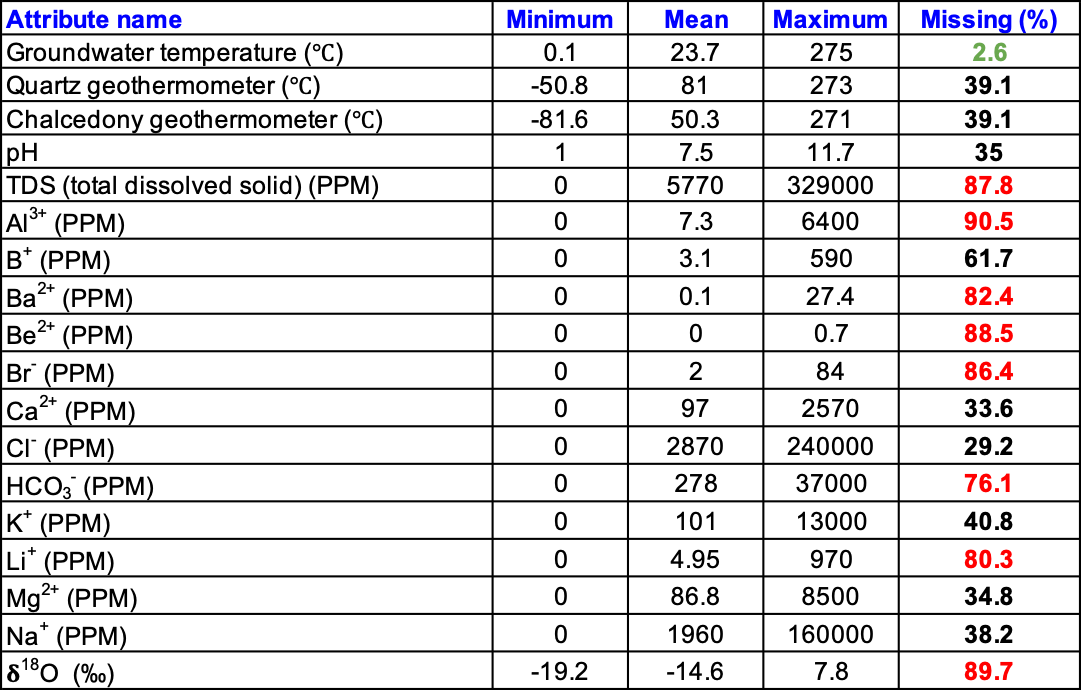
\includegraphics{../data/gb_duplicatedRows.png}
\caption{gb\_duplicatedRows}
\end{figure}

Close to complete records are available only for \texttt{Temperature}.

Data for \texttt{TDS}, \texttt{Al} and \texttt{δO18} are heavily
missing.

Even though, the dataset is very sparse, our ML methods can analyze the
inputs.

Most of the commonly used ML methods cannot process datasets that are
sparse.

    \hypertarget{log-transformation}{%
\subsubsection{Log-transformation}\label{log-transformation}}

Attribute values are log-transformed to better capture the order of
magnitude variability.

All attributes execpt for \texttt{Quartz}, \texttt{Chalcedony} and
\texttt{pH} are log-transformed.

    \begin{tcolorbox}[breakable, size=fbox, boxrule=1pt, pad at break*=1mm,colback=cellbackground, colframe=cellborder]
\prompt{In}{incolor}{8}{\boxspacing}
\begin{Verbatim}[commandchars=\\\{\}]
\PY{n}{logv} \PY{o}{=} \PY{p}{[}\PY{k+kc}{true}\PY{p}{,} \PY{k+kc}{false}\PY{p}{,} \PY{k+kc}{false}\PY{p}{,} \PY{k+kc}{false}\PY{p}{,}  \PY{k+kc}{true}\PY{p}{,} \PY{k+kc}{true}\PY{p}{,} \PY{k+kc}{true}\PY{p}{,} \PY{k+kc}{true}\PY{p}{,} \PY{k+kc}{true}\PY{p}{,} \PY{k+kc}{true}\PY{p}{,} \PY{k+kc}{true}\PY{p}{,} \PY{k+kc}{true}\PY{p}{,} \PY{k+kc}{true}\PY{p}{,} \PY{k+kc}{true}\PY{p}{,} \PY{k+kc}{true}\PY{p}{,} \PY{k+kc}{true}\PY{p}{,} \PY{k+kc}{true}\PY{p}{,} \PY{k+kc}{true}\PY{p}{]}
\PY{p}{[}\PY{n}{attributes} \PY{n}{logv}\PY{p}{]}
\end{Verbatim}
\end{tcolorbox}

            \begin{tcolorbox}[breakable, size=fbox, boxrule=.5pt, pad at break*=1mm, opacityfill=0]
\prompt{Out}{outcolor}{8}{\boxspacing}
\begin{Verbatim}[commandchars=\\\{\}]
18×2 Array\{Any,2\}:
 "Temperature"   true
 "Quartz"       false
 "Chalcedony"   false
 "pH"           false
 "TDS"           true
 "Al"            true
 "B"             true
 "Ba"            true
 "Be"            true
 "Br"            true
 "Ca"            true
 "Cl"            true
 "HCO3"          true
 "K"             true
 "Li"            true
 "Mg"            true
 "Na"            true
 "δO18"          true
\end{Verbatim}
\end{tcolorbox}
        
    \begin{tcolorbox}[breakable, size=fbox, boxrule=1pt, pad at break*=1mm,colback=cellbackground, colframe=cellborder]
\prompt{In}{incolor}{9}{\boxspacing}
\begin{Verbatim}[commandchars=\\\{\}]
\PY{n}{NMFk}\PY{o}{.}\PY{n}{datanalytics}\PY{p}{(}\PY{n}{X}\PY{p}{,} \PY{n}{attributes}\PY{p}{;} \PY{n}{dims}\PY{o}{=}\PY{l+m+mi}{2}\PY{p}{,} \PY{n}{logv}\PY{o}{=}\PY{n}{logv}\PY{p}{)}\PY{p}{;}
\end{Verbatim}
\end{tcolorbox}

    \begin{center}
    \adjustimage{max size={0.9\linewidth}{0.9\paperheight}}{GreatBasin_files/GreatBasin_21_0.png}
    \end{center}
    { \hspace*{\fill} \\}
    
    \begin{Verbatim}[commandchars=\\\{\}]
┌ Info: Temperature: log10-transformed
└ @ NMFk /Users/vvv/.julia/dev/NMFk/src/NMFkPreprocess.jl:51
    \end{Verbatim}

    \begin{center}
    \adjustimage{max size={0.9\linewidth}{0.9\paperheight}}{GreatBasin_files/GreatBasin_21_2.png}
    \end{center}
    { \hspace*{\fill} \\}
    
    \begin{center}
    \adjustimage{max size={0.9\linewidth}{0.9\paperheight}}{GreatBasin_files/GreatBasin_21_3.png}
    \end{center}
    { \hspace*{\fill} \\}
    
    \begin{Verbatim}[commandchars=\\\{\}]
Temperature: Min -1.0 Max 2.4393327 StdDev 0.28062904 Skewness 0.8823397 Count
13894
Quartz: Min -50.870045 Max 273.2438 StdDev 34.105637 Skewness 0.6946969 Count
8683
    \end{Verbatim}

    \begin{Verbatim}[commandchars=\\\{\}]
┌ Info: Quartz
└ @ NMFk /Users/vvv/.julia/dev/NMFk/src/NMFkPreprocess.jl:54
┌ Info: Chalcedony
└ @ NMFk /Users/vvv/.julia/dev/NMFk/src/NMFkPreprocess.jl:54
    \end{Verbatim}

    \begin{center}
    \adjustimage{max size={0.9\linewidth}{0.9\paperheight}}{GreatBasin_files/GreatBasin_21_6.png}
    \end{center}
    { \hspace*{\fill} \\}
    
    \begin{center}
    \adjustimage{max size={0.9\linewidth}{0.9\paperheight}}{GreatBasin_files/GreatBasin_21_7.png}
    \end{center}
    { \hspace*{\fill} \\}
    
    \begin{Verbatim}[commandchars=\\\{\}]
Chalcedony: Min -81.64773 Max 271.23828 StdDev 36.418324 Skewness 0.8679946
Count 8683
pH: Min 1.0 Max 11.7 StdDev 0.55800503 Skewness -0.5521828 Count 9261
    \end{Verbatim}

    \begin{Verbatim}[commandchars=\\\{\}]
┌ Info: pH
└ @ NMFk /Users/vvv/.julia/dev/NMFk/src/NMFkPreprocess.jl:54
┌ Info: TDS: log10-transformed
└ @ NMFk /Users/vvv/.julia/dev/NMFk/src/NMFkPreprocess.jl:51
    \end{Verbatim}

    \begin{center}
    \adjustimage{max size={0.9\linewidth}{0.9\paperheight}}{GreatBasin_files/GreatBasin_21_10.png}
    \end{center}
    { \hspace*{\fill} \\}
    
    \begin{center}
    \adjustimage{max size={0.9\linewidth}{0.9\paperheight}}{GreatBasin_files/GreatBasin_21_11.png}
    \end{center}
    { \hspace*{\fill} \\}
    
    \begin{Verbatim}[commandchars=\\\{\}]
TDS: Min -2.6989698 Max 5.5171957 StdDev 2.0129914 Skewness -1.7111415 Count
1740
Al: Min -5.8860564 Max 3.80618 StdDev 1.2161667 Skewness -0.44271475 Count 1362
    \end{Verbatim}

    \begin{Verbatim}[commandchars=\\\{\}]
┌ Info: Al: log10-transformed
└ @ NMFk /Users/vvv/.julia/dev/NMFk/src/NMFkPreprocess.jl:51
┌ Info: B: log10-transformed
└ @ NMFk /Users/vvv/.julia/dev/NMFk/src/NMFkPreprocess.jl:51
    \end{Verbatim}

    \begin{center}
    \adjustimage{max size={0.9\linewidth}{0.9\paperheight}}{GreatBasin_files/GreatBasin_21_14.png}
    \end{center}
    { \hspace*{\fill} \\}
    
    \begin{Verbatim}[commandchars=\\\{\}]
B: Min -4.0 Max 2.770852 StdDev 0.99189556 Skewness -0.15991572 Count 5462
    \end{Verbatim}

    \begin{Verbatim}[commandchars=\\\{\}]
┌ Info: Ba: log10-transformed
└ @ NMFk /Users/vvv/.julia/dev/NMFk/src/NMFkPreprocess.jl:51
    \end{Verbatim}

    \begin{center}
    \adjustimage{max size={0.9\linewidth}{0.9\paperheight}}{GreatBasin_files/GreatBasin_21_17.png}
    \end{center}
    { \hspace*{\fill} \\}
    
    \begin{center}
    \adjustimage{max size={0.9\linewidth}{0.9\paperheight}}{GreatBasin_files/GreatBasin_21_18.png}
    \end{center}
    { \hspace*{\fill} \\}
    
    \begin{Verbatim}[commandchars=\\\{\}]
Ba: Min -4.0 Max 1.4382393 StdDev 0.492002 Skewness -0.63361335 Count 2516
Be: Min -8.0 Max -0.15490197 StdDev 0.8196359 Skewness -2.5543597 Count 1640
    \end{Verbatim}

    \begin{Verbatim}[commandchars=\\\{\}]
┌ Info: Be: log10-transformed
└ @ NMFk /Users/vvv/.julia/dev/NMFk/src/NMFkPreprocess.jl:51
┌ Info: Br: log10-transformed
└ @ NMFk /Users/vvv/.julia/dev/NMFk/src/NMFkPreprocess.jl:51
    \end{Verbatim}

    \begin{center}
    \adjustimage{max size={0.9\linewidth}{0.9\paperheight}}{GreatBasin_files/GreatBasin_21_21.png}
    \end{center}
    { \hspace*{\fill} \\}
    
    \begin{Verbatim}[commandchars=\\\{\}]
Br: Min -3.102373 Max 1.9242793 StdDev 0.90064573 Skewness 0.497394 Count 1935
    \end{Verbatim}

    \begin{Verbatim}[commandchars=\\\{\}]
┌ Info: Ca: log10-transformed
└ @ NMFk /Users/vvv/.julia/dev/NMFk/src/NMFkPreprocess.jl:51
    \end{Verbatim}

    \begin{center}
    \adjustimage{max size={0.9\linewidth}{0.9\paperheight}}{GreatBasin_files/GreatBasin_21_24.png}
    \end{center}
    { \hspace*{\fill} \\}
    
    \begin{center}
    \adjustimage{max size={0.9\linewidth}{0.9\paperheight}}{GreatBasin_files/GreatBasin_21_25.png}
    \end{center}
    { \hspace*{\fill} \\}
    
    \begin{Verbatim}[commandchars=\\\{\}]
Ca: Min -2.0 Max 3.4093695 StdDev 0.51392627 Skewness -0.4936186 Count 9468
Cl: Min -4.0 Max 5.3802114 StdDev 0.99255455 Skewness 0.45536557 Count 10091
    \end{Verbatim}

    \begin{Verbatim}[commandchars=\\\{\}]
┌ Info: Cl: log10-transformed
└ @ NMFk /Users/vvv/.julia/dev/NMFk/src/NMFkPreprocess.jl:51
┌ Info: HCO3: log10-transformed
└ @ NMFk /Users/vvv/.julia/dev/NMFk/src/NMFkPreprocess.jl:51
    \end{Verbatim}

    \begin{center}
    \adjustimage{max size={0.9\linewidth}{0.9\paperheight}}{GreatBasin_files/GreatBasin_21_28.png}
    \end{center}
    { \hspace*{\fill} \\}
    
    \begin{Verbatim}[commandchars=\\\{\}]
HCO3: Min -1.0 Max 4.5682015 StdDev 0.36140293 Skewness -0.94632554 Count 3413
    \end{Verbatim}

    \begin{Verbatim}[commandchars=\\\{\}]
┌ Info: K: log10-transformed
└ @ NMFk /Users/vvv/.julia/dev/NMFk/src/NMFkPreprocess.jl:51
    \end{Verbatim}

    \begin{center}
    \adjustimage{max size={0.9\linewidth}{0.9\paperheight}}{GreatBasin_files/GreatBasin_21_31.png}
    \end{center}
    { \hspace*{\fill} \\}
    
    \begin{Verbatim}[commandchars=\\\{\}]
K: Min -2.09691 Max 4.1139436 StdDev 0.686127 Skewness 1.5732428 Count 8446
    \end{Verbatim}

    \begin{Verbatim}[commandchars=\\\{\}]
┌ Info: Li: log10-transformed
└ @ NMFk /Users/vvv/.julia/dev/NMFk/src/NMFkPreprocess.jl:51
    \end{Verbatim}

    \begin{center}
    \adjustimage{max size={0.9\linewidth}{0.9\paperheight}}{GreatBasin_files/GreatBasin_21_34.png}
    \end{center}
    { \hspace*{\fill} \\}
    
    \begin{center}
    \adjustimage{max size={0.9\linewidth}{0.9\paperheight}}{GreatBasin_files/GreatBasin_21_35.png}
    \end{center}
    { \hspace*{\fill} \\}
    
    \begin{Verbatim}[commandchars=\\\{\}]
Li: Min -6.0 Max 2.9867718 StdDev 1.2346249 Skewness -0.6840743 Count 2809
Mg: Min -3.69897 Max 3.929419 StdDev 0.79547274 Skewness -1.0883808 Count 9296
    \end{Verbatim}

    \begin{Verbatim}[commandchars=\\\{\}]
┌ Info: Mg: log10-transformed
└ @ NMFk /Users/vvv/.julia/dev/NMFk/src/NMFkPreprocess.jl:51
┌ Info: Na: log10-transformed
└ @ NMFk /Users/vvv/.julia/dev/NMFk/src/NMFkPreprocess.jl:51
    \end{Verbatim}

    \begin{center}
    \adjustimage{max size={0.9\linewidth}{0.9\paperheight}}{GreatBasin_files/GreatBasin_21_38.png}
    \end{center}
    { \hspace*{\fill} \\}
    
    \begin{Verbatim}[commandchars=\\\{\}]
Na: Min -1.6989701 Max 5.20412 StdDev 0.8328025 Skewness 1.1553397 Count 8814
δO18: Min -0.096910425 Max 1.4448252 StdDev 0.20046535 Skewness 0.21996279 Count
1471
Name Min Max StdDev Count (non-NaN's)
Temperature -1.0 2.4393327 0.28062904 0.8823397 13894
Quartz -50.870045 273.2438 34.105637 0.6946969 8683
Chalcedony -81.64773 271.23828 36.418324 0.8679946 8683
pH 1.0 11.7 0.55800503 -0.5521828 9261
TDS -2.6989698 5.5171957 2.0129914 -1.7111415 1740
Al -5.8860564 3.80618 1.2161667 -0.44271475 1362
B -4.0 2.770852 0.99189556 -0.15991572 5462
Ba -4.0 1.4382393 0.492002 -0.63361335 2516
Be -8.0 -0.15490197 0.8196359 -2.5543597 1640
Br -3.102373 1.9242793 0.90064573 0.497394 1935
Ca -2.0 3.4093695 0.51392627 -0.4936186 9468
Cl -4.0 5.3802114 0.99255455 0.45536557 10091
HCO3 -1.0 4.5682015 0.36140293 -0.94632554 3413
K -2.09691 4.1139436 0.686127 1.5732428 8446
Li -6.0 2.9867718 1.2346249 -0.6840743 2809
Mg -3.69897 3.929419 0.79547274 -1.0883808 9296
Na -1.6989701 5.20412 0.8328025 1.1553397 8814
δO18 -0.096910425 1.4448252 0.20046535 0.21996279 1471
    \end{Verbatim}

    \begin{Verbatim}[commandchars=\\\{\}]
┌ Info: δO18: log10-transformed
└ @ NMFk /Users/vvv/.julia/dev/NMFk/src/NMFkPreprocess.jl:51
┌ Info: Attributes
└ @ NMFk /Users/vvv/.julia/dev/NMFk/src/NMFkPreprocess.jl:70
    \end{Verbatim}

    \hypertarget{define-and-normalize-the-data-matrix}{%
\paragraph{Define and normalize the data
matrix}\label{define-and-normalize-the-data-matrix}}

    \begin{tcolorbox}[breakable, size=fbox, boxrule=1pt, pad at break*=1mm,colback=cellbackground, colframe=cellborder]
\prompt{In}{incolor}{10}{\boxspacing}
\begin{Verbatim}[commandchars=\\\{\}]
\PY{n}{Xnl}\PY{p}{,} \PY{n}{xlmin}\PY{p}{,} \PY{n}{xlmax}\PY{p}{,} \PY{n}{zflag} \PY{o}{=} \PY{n}{NMFk}\PY{o}{.}\PY{n}{normalizematrix\PYZus{}col}\PY{p}{(}\PY{n}{X}\PY{p}{;} \PY{n}{logv}\PY{o}{=}\PY{n}{logv}\PY{p}{)}\PY{p}{;}
\end{Verbatim}
\end{tcolorbox}

    \hypertarget{define-a-range-for-number-of-signatures-to-be-explored}{%
\subsubsection{Define a range for number of signatures to be
explored}\label{define-a-range-for-number-of-signatures-to-be-explored}}

    \begin{tcolorbox}[breakable, size=fbox, boxrule=1pt, pad at break*=1mm,colback=cellbackground, colframe=cellborder]
\prompt{In}{incolor}{11}{\boxspacing}
\begin{Verbatim}[commandchars=\\\{\}]
\PY{n}{nkrange} \PY{o}{=} \PY{l+m+mi}{2}\PY{o}{:}\PY{l+m+mi}{10}\PY{p}{;}
\end{Verbatim}
\end{tcolorbox}

    \hypertarget{define-directory-with-exsiting-model-runs}{%
\subsubsection{Define directory with exsiting model
runs}\label{define-directory-with-exsiting-model-runs}}

    \begin{tcolorbox}[breakable, size=fbox, boxrule=1pt, pad at break*=1mm,colback=cellbackground, colframe=cellborder]
\prompt{In}{incolor}{12}{\boxspacing}
\begin{Verbatim}[commandchars=\\\{\}]
\PY{n}{resultdir} \PY{o}{=} \PY{l+s}{\PYZdq{}}\PY{l+s}{r}\PY{l+s}{e}\PY{l+s}{s}\PY{l+s}{u}\PY{l+s}{l}\PY{l+s}{t}\PY{l+s}{s}\PY{l+s}{\PYZdq{}}\PY{p}{;}
\end{Verbatim}
\end{tcolorbox}

    \hypertarget{define-the-number-of-nmf-runs-to-be-exectuted}{%
\paragraph{Define the number of NMF runs to be
exectuted}\label{define-the-number-of-nmf-runs-to-be-exectuted}}

The higher the NMF runs, the better. In addition, convergence has been
already explored using different numbers of NMF runs.

    \begin{tcolorbox}[breakable, size=fbox, boxrule=1pt, pad at break*=1mm,colback=cellbackground, colframe=cellborder]
\prompt{In}{incolor}{13}{\boxspacing}
\begin{Verbatim}[commandchars=\\\{\}]
\PY{n}{nruns} \PY{o}{=} \PY{l+m+mi}{640}\PY{p}{;}
\end{Verbatim}
\end{tcolorbox}

    \hypertarget{perform-ml-analyses}{%
\subsection{Perform ML analyses}\label{perform-ml-analyses}}

The \textbf{NMFk} algorithm factorizes the normalized data matrix
\texttt{Xn} into \texttt{W} and \texttt{H} matrices. For more
information, check out the
\href{https://github.com/SmartTensors/NMFk.jl}{\textbf{NMFk} website}

    \begin{tcolorbox}[breakable, size=fbox, boxrule=1pt, pad at break*=1mm,colback=cellbackground, colframe=cellborder]
\prompt{In}{incolor}{14}{\boxspacing}
\begin{Verbatim}[commandchars=\\\{\}]
\PY{n}{W}\PY{p}{,} \PY{n}{H}\PY{p}{,} \PY{n}{fitquality}\PY{p}{,} \PY{n}{robustness}\PY{p}{,} \PY{n}{aic} \PY{o}{=} \PY{n}{NMFk}\PY{o}{.}\PY{n}{execute}\PY{p}{(}\PY{n}{Xnl}\PY{p}{,} \PY{n}{nkrange}\PY{p}{,} \PY{n}{nruns}\PY{p}{;} \PY{n}{resultdir}\PY{o}{=}\PY{n}{resultdir}\PY{p}{,} \PY{n}{casefilename}\PY{o}{=}\PY{l+s}{\PYZdq{}}\PY{l+s}{n}\PY{l+s}{m}\PY{l+s}{f}\PY{l+s}{k}\PY{l+s}{\PYZhy{}}\PY{l+s}{n}\PY{l+s}{l}\PY{l+s}{\PYZdq{}}\PY{p}{,} \PY{n}{load}\PY{o}{=}\PY{k+kc}{true}\PY{p}{)}
\PY{n}{W}\PY{p}{,} \PY{n}{H}\PY{p}{,} \PY{n}{fitquality}\PY{p}{,} \PY{n}{robustness}\PY{p}{,} \PY{n}{aic} \PY{o}{=} \PY{n}{NMFk}\PY{o}{.}\PY{n}{load}\PY{p}{(}\PY{n}{nkrange}\PY{p}{,} \PY{n}{nruns}\PY{p}{;} \PY{n}{resultdir}\PY{o}{=}\PY{n}{resultdir}\PY{p}{,} \PY{n}{casefilename}\PY{o}{=}\PY{l+s}{\PYZdq{}}\PY{l+s}{n}\PY{l+s}{m}\PY{l+s}{f}\PY{l+s}{k}\PY{l+s}{\PYZhy{}}\PY{l+s}{n}\PY{l+s}{l}\PY{l+s}{\PYZdq{}}\PY{p}{)}\PY{p}{;}
\end{Verbatim}
\end{tcolorbox}

    \begin{Verbatim}[commandchars=\\\{\}]
Signals:  2 Fit:     490.2203 Silhouette:     0.886031 AIC:    -531856.6
Signals:  3 Fit:     315.1114 Silhouette:     0.498339 AIC:    -551467.8
Signals:  4 Fit:      224.617 Silhouette:  -0.01242121 AIC:    -559810.1
Signals:  5 Fit:     157.1487 Silhouette:  0.004662591 AIC:    -570187.6
Signals:  6 Fit:     118.4444 Silhouette:   -0.1862046 AIC:    -572450.7
Signals:  7 Fit:      85.8435 Silhouette:  -0.09372894 AIC:    -578982.6
Signals:  8 Fit:      62.9881 Silhouette:    -0.113508 AIC:    -584169.8
Signals:  9 Fit:     45.59955 Silhouette:  -0.05323793 AIC:    -590824.9
Signals: 10 Fit:     33.40136 Silhouette:  -0.08453866 AIC:    -596199.8
Signals:  2 Fit:     490.2203 Silhouette:     0.886031 AIC:    -531856.6
Signals:  3 Fit:     315.1114 Silhouette:     0.498339 AIC:    -551467.8
Signals:  4 Fit:      224.617 Silhouette:  -0.01242121 AIC:    -559810.1
Signals:  5 Fit:     157.1487 Silhouette:  0.004662591 AIC:    -570187.6
Signals:  6 Fit:     118.4444 Silhouette:   -0.1862046 AIC:    -572450.7
Signals:  7 Fit:      85.8435 Silhouette:  -0.09372894 AIC:    -578982.6
Signals:  8 Fit:      62.9881 Silhouette:    -0.113508 AIC:    -584169.8
Signals:  9 Fit:     45.59955 Silhouette:  -0.05323793 AIC:    -590824.9
Signals: 10 Fit:     33.40136 Silhouette:  -0.08453866 AIC:    -596199.8
Signals:  2 Fit:     490.2203 Silhouette:     0.886031 AIC:    -531856.6
Signals:  3 Fit:     315.1114 Silhouette:     0.498339 AIC:    -551467.8
Signals:  4 Fit:      224.617 Silhouette:  -0.01242121 AIC:    -559810.1
Signals:  5 Fit:     157.1487 Silhouette:  0.004662591 AIC:    -570187.6
Signals:  6 Fit:     118.4444 Silhouette:   -0.1862046 AIC:    -572450.7
Signals:  7 Fit:      85.8435 Silhouette:  -0.09372894 AIC:    -578982.6
Signals:  8 Fit:      62.9881 Silhouette:    -0.113508 AIC:    -584169.8
Signals:  9 Fit:     45.59955 Silhouette:  -0.05323793 AIC:    -590824.9
Signals: 10 Fit:     33.40136 Silhouette:  -0.08453866 AIC:    -596199.8
    \end{Verbatim}

    \begin{Verbatim}[commandchars=\\\{\}]
┌ Info: Results
└ @ NMFk /Users/vvv/.julia/dev/NMFk/src/NMFkExecute.jl:15
┌ Info: Optimal solution: 3 signals
└ @ NMFk /Users/vvv/.julia/dev/NMFk/src/NMFkExecute.jl:20
┌ Info: Optimal solution: 3 signals
└ @ NMFk /Users/vvv/.julia/dev/NMFk/src/NMFkIO.jl:30
    \end{Verbatim}

    Here, the \textbf{NMFk} results are loaded from a prior ML run.

As seen from the output above, the NMFk analyses identified that the
optimal number of geothermal signatures in the dataset \textbf{3}.

Solutions with a number of signatures less than \textbf{3} are
underfitting.

Solutions with a number of signatures greater than \textbf{3} are
overfitting and unacceptable.

The set of acceptable solutions are defined as follows:

    \begin{tcolorbox}[breakable, size=fbox, boxrule=1pt, pad at break*=1mm,colback=cellbackground, colframe=cellborder]
\prompt{In}{incolor}{15}{\boxspacing}
\begin{Verbatim}[commandchars=\\\{\}]
\PY{n}{NMFk}\PY{o}{.}\PY{n}{getks}\PY{p}{(}\PY{n}{nkrange}\PY{p}{,} \PY{n}{robustness}\PY{p}{[}\PY{n}{nkrange}\PY{p}{]}\PY{p}{)}
\end{Verbatim}
\end{tcolorbox}

            \begin{tcolorbox}[breakable, size=fbox, boxrule=.5pt, pad at break*=1mm, opacityfill=0]
\prompt{Out}{outcolor}{15}{\boxspacing}
\begin{Verbatim}[commandchars=\\\{\}]
2-element Array\{Int64,1\}:
 2
 3
\end{Verbatim}
\end{tcolorbox}
        
    The acceptable solutions contain 2 and 3 signatures.

    \hypertarget{post-processing-nmfk-results}{%
\subsubsection{Post-processing NMFk
results}\label{post-processing-nmfk-results}}

\hypertarget{number-of-signatures}{%
\paragraph{Number of signatures}\label{number-of-signatures}}

Plot representing solution quality (fit) and silhouette width
(robustness) for different number of signatures \texttt{k}:

    \begin{tcolorbox}[breakable, size=fbox, boxrule=1pt, pad at break*=1mm,colback=cellbackground, colframe=cellborder]
\prompt{In}{incolor}{16}{\boxspacing}
\begin{Verbatim}[commandchars=\\\{\}]
\PY{n}{resultdirpost} \PY{o}{=} \PY{l+s}{\PYZdq{}}\PY{l+s}{r}\PY{l+s}{e}\PY{l+s}{s}\PY{l+s}{u}\PY{l+s}{l}\PY{l+s}{t}\PY{l+s}{s}\PY{l+s}{\PYZhy{}}\PY{l+s}{p}\PY{l+s}{o}\PY{l+s}{s}\PY{l+s}{t}\PY{l+s}{p}\PY{l+s}{r}\PY{l+s}{o}\PY{l+s}{c}\PY{l+s}{e}\PY{l+s}{s}\PY{l+s}{s}\PY{l+s}{i}\PY{l+s}{n}\PY{l+s}{g}\PY{l+s}{\PYZhy{}}\PY{l+s}{n}\PY{l+s}{l}\PY{l+s}{\PYZhy{}}\PY{l+s+si}{\PYZdl{}}\PY{p}{(}\PY{n}{nruns}\PY{p}{)}\PY{l+s}{\PYZdq{}}
\PY{n}{figuredirpost} \PY{o}{=} \PY{l+s}{\PYZdq{}}\PY{l+s}{f}\PY{l+s}{i}\PY{l+s}{g}\PY{l+s}{u}\PY{l+s}{r}\PY{l+s}{e}\PY{l+s}{s}\PY{l+s}{\PYZhy{}}\PY{l+s}{p}\PY{l+s}{o}\PY{l+s}{s}\PY{l+s}{t}\PY{l+s}{p}\PY{l+s}{r}\PY{l+s}{o}\PY{l+s}{c}\PY{l+s}{e}\PY{l+s}{s}\PY{l+s}{s}\PY{l+s}{i}\PY{l+s}{n}\PY{l+s}{g}\PY{l+s}{\PYZhy{}}\PY{l+s}{n}\PY{l+s}{l}\PY{l+s}{\PYZhy{}}\PY{l+s+si}{\PYZdl{}}\PY{p}{(}\PY{n}{nruns}\PY{p}{)}\PY{l+s}{\PYZdq{}}\PY{p}{;}
\end{Verbatim}
\end{tcolorbox}

    \begin{tcolorbox}[breakable, size=fbox, boxrule=1pt, pad at break*=1mm,colback=cellbackground, colframe=cellborder]
\prompt{In}{incolor}{17}{\boxspacing}
\begin{Verbatim}[commandchars=\\\{\}]
\PY{n}{NMFk}\PY{o}{.}\PY{n}{plot\PYZus{}feature\PYZus{}selecton}\PY{p}{(}\PY{n}{nkrange}\PY{p}{,} \PY{n}{fitquality}\PY{p}{,} \PY{n}{robustness}\PY{p}{;} \PY{n}{figuredir}\PY{o}{=}\PY{n}{figuredirpost}\PY{p}{)}
\end{Verbatim}
\end{tcolorbox}

    \begin{center}
    \adjustimage{max size={0.9\linewidth}{0.9\paperheight}}{GreatBasin_files/GreatBasin_37_0.png}
    \end{center}
    { \hspace*{\fill} \\}
    
    \begin{Verbatim}[commandchars=\\\{\}]

    \end{Verbatim}

    The plot above also demonstrates that the accceptable solutions contain
2 and 3 signatures. Note, any solution is accepted, if the robustness
\textgreater0.25.

\hypertarget{analysis-of-the-optimal-solution}{%
\paragraph{Analysis of the optimal
solution}\label{analysis-of-the-optimal-solution}}

The ML solution with the optimal number of signatures (3) is further
analyzed as follows:

    \begin{tcolorbox}[breakable, size=fbox, boxrule=1pt, pad at break*=1mm,colback=cellbackground, colframe=cellborder]
\prompt{In}{incolor}{18}{\boxspacing}
\begin{Verbatim}[commandchars=\\\{\}]
\PY{n}{Sorder}\PY{p}{,} \PY{n}{Wclusters}\PY{p}{,} \PY{n}{Hclusters} \PY{o}{=} \PY{n}{NMFk}\PY{o}{.}\PY{n}{clusterresults}\PY{p}{(}\PY{n}{NMFk}\PY{o}{.}\PY{n}{getk}\PY{p}{(}\PY{n}{nkrange}\PY{p}{,} \PY{n}{robustness}\PY{p}{[}\PY{n}{nkrange}\PY{p}{]}\PY{p}{)}\PY{p}{,} \PY{n}{W}\PY{p}{,} \PY{n}{H}\PY{p}{,} \PY{n}{string}\PY{o}{.}\PY{p}{(}\PY{n}{collect}\PY{p}{(}\PY{l+m+mi}{1}\PY{o}{:}\PY{n}{npoints}\PY{p}{)}\PY{p}{)}\PY{p}{,} \PY{n}{attributes}\PY{p}{;} \PY{n}{lon}\PY{o}{=}\PY{n}{xcoord}\PY{p}{,} \PY{n}{lat}\PY{o}{=}\PY{n}{ycoord}\PY{p}{,} \PY{n}{resultdir}\PY{o}{=}\PY{n}{resultdirpost}\PY{p}{,} \PY{n}{figuredir}\PY{o}{=}\PY{n}{figuredirpost}\PY{p}{,} \PY{n}{ordersignal}\PY{o}{=}\PY{o}{:}\PY{n}{Wcount}\PY{p}{,} \PY{n}{Hcasefilename}\PY{o}{=}\PY{l+s}{\PYZdq{}}\PY{l+s}{a}\PY{l+s}{t}\PY{l+s}{t}\PY{l+s}{r}\PY{l+s}{i}\PY{l+s}{b}\PY{l+s}{u}\PY{l+s}{t}\PY{l+s}{e}\PY{l+s}{s}\PY{l+s}{\PYZdq{}}\PY{p}{,} \PY{n}{Wcasefilename}\PY{o}{=}\PY{l+s}{\PYZdq{}}\PY{l+s}{l}\PY{l+s}{o}\PY{l+s}{c}\PY{l+s}{a}\PY{l+s}{t}\PY{l+s}{i}\PY{l+s}{o}\PY{l+s}{n}\PY{l+s}{s}\PY{l+s}{\PYZdq{}}\PY{p}{,} \PY{n}{biplotcolor}\PY{o}{=}\PY{o}{:}\PY{n}{WH}\PY{p}{,} \PY{n}{sortmag}\PY{o}{=}\PY{k+kc}{false}\PY{p}{,} \PY{n}{biplotlabel}\PY{o}{=}\PY{o}{:}\PY{n}{H}\PY{p}{,} \PY{n}{point\PYZus{}size\PYZus{}nolabel}\PY{o}{=}\PY{l+m+mi}{2}\PY{n}{Gadfly}\PY{o}{.}\PY{n}{pt}\PY{p}{,} \PY{n}{point\PYZus{}size\PYZus{}label}\PY{o}{=}\PY{l+m+mi}{4}\PY{n}{Gadfly}\PY{o}{.}\PY{n}{pt}\PY{p}{)}
\end{Verbatim}
\end{tcolorbox}

    \begin{Verbatim}[commandchars=\\\{\}]
Signal importance (high->low): [2, 1, 3]
    \end{Verbatim}

    \begin{Verbatim}[commandchars=\\\{\}]
┌ Info: Number of signals: 3
└ @ NMFk /Users/vvv/.julia/dev/NMFk/src/NMFkPostprocess.jl:154
┌ Info: Attributes (signals=3)
└ @ NMFk /Users/vvv/.julia/dev/NMFk/src/NMFkPostprocess.jl:158
┌ Warning: type
Clustering.KmeansResult\{Core.Array\{Core.Float32,2\},Core.Float32,Core.Int64\} not
present in workspace; reconstructing
└ @ JLD /Users/vvv/.julia/packages/JLD/nQ9iW/src/jld\_types.jl:697
┌ Info: Robust k-means analysis results are loaded from file results-
postprocessing-nl-640/Hmatrix-3-3\_18-1000.jld!
└ @ NMFk /Users/vvv/.julia/dev/NMFk/src/NMFkCluster.jl:67
┌ Warning: Procedure to find unique signals could not identify a solution {\ldots}
└ @ NMFk /Users/vvv/.julia/dev/NMFk/src/NMFkCluster.jl:158
┌ Warning: Procedure to find unique signals could not identify a solution {\ldots}
└ @ NMFk /Users/vvv/.julia/dev/NMFk/src/NMFkCluster.jl:158
┌ Warning: Procedure to find unique signals could not identify a solution {\ldots}
└ @ NMFk /Users/vvv/.julia/dev/NMFk/src/NMFkCluster.jl:158
┌ Warning: type
Clustering.KmeansResult\{Core.Array\{Core.Float32,2\},Core.Float32,Core.Int64\} not
present in workspace; reconstructing
└ @ JLD /Users/vvv/.julia/packages/JLD/nQ9iW/src/jld\_types.jl:697
┌ Info: Robust k-means analysis results are loaded from file results-
postprocessing-nl-640/Wmatrix-3-3\_14258-1000.jld!
└ @ NMFk /Users/vvv/.julia/dev/NMFk/src/NMFkCluster.jl:67
┌ Warning: Procedure to find unique signals could not identify a solution {\ldots}
└ @ NMFk /Users/vvv/.julia/dev/NMFk/src/NMFkCluster.jl:158
┌ Warning: Procedure to find unique signals could not identify a solution {\ldots}
└ @ NMFk /Users/vvv/.julia/dev/NMFk/src/NMFkCluster.jl:158
    \end{Verbatim}

    
    \begin{Verbatim}[commandchars=\\\{\}]
8×2 Array\{Any,2\}:
 "Br"    1.0
 "TDS"   0.998519
 "B"     0.761876
 "δO18"  0.63782
 "Na"    0.548602
 "Li"    0.463867
 "Cl"    0.457713
 "K"     0.427433
    \end{Verbatim}

    
    \begin{Verbatim}[commandchars=\\\{\}]
┌ Info: Signal A -> A Count: 8
└ @ NMFk /Users/vvv/.julia/dev/NMFk/src/NMFkPostprocess.jl:265
┌ Info: Signal C -> B Count: 3
└ @ NMFk /Users/vvv/.julia/dev/NMFk/src/NMFkPostprocess.jl:265
┌ Info: Signal B -> C Count: 7
└ @ NMFk /Users/vvv/.julia/dev/NMFk/src/NMFkPostprocess.jl:265
┌ Info: Signal A (S3) (k-means clustering)
└ @ NMFk /Users/vvv/.julia/dev/NMFk/src/NMFkPostprocess.jl:282
    \end{Verbatim}

    
    \begin{Verbatim}[commandchars=\\\{\}]
3×2 Array\{Any,2\}:
 "Quartz"      1.0
 "Chalcedony"  0.945545
 "Al"          0.802297
    \end{Verbatim}

    
    
    \begin{Verbatim}[commandchars=\\\{\}]
7×2 Array\{Any,2\}:
 "Mg"           1.0
 "Ca"           0.935713
 "HCO3"         0.679563
 "pH"           0.651626
 "Ba"           0.622107
 "Be"           0.578012
 "Temperature"  0.464707
    \end{Verbatim}

    
    \begin{center}
    \adjustimage{max size={0.9\linewidth}{0.9\paperheight}}{GreatBasin_files/GreatBasin_39_6.png}
    \end{center}
    { \hspace*{\fill} \\}
    
    \begin{Verbatim}[commandchars=\\\{\}]
┌ Info: Signal B (S1) (k-means clustering)
└ @ NMFk /Users/vvv/.julia/dev/NMFk/src/NMFkPostprocess.jl:282
┌ Info: Signal C (S2) (k-means clustering)
└ @ NMFk /Users/vvv/.julia/dev/NMFk/src/NMFkPostprocess.jl:282
    \end{Verbatim}

    \begin{center}
    \adjustimage{max size={0.9\linewidth}{0.9\paperheight}}{GreatBasin_files/GreatBasin_39_8.png}
    \end{center}
    { \hspace*{\fill} \\}
    
    \begin{Verbatim}[commandchars=\\\{\}]

    \end{Verbatim}

    \begin{center}
    \adjustimage{max size={0.9\linewidth}{0.9\paperheight}}{GreatBasin_files/GreatBasin_39_10.png}
    \end{center}
    { \hspace*{\fill} \\}
    
    \begin{center}
    \adjustimage{max size={0.9\linewidth}{0.9\paperheight}}{GreatBasin_files/GreatBasin_39_11.png}
    \end{center}
    { \hspace*{\fill} \\}
    
    \begin{Verbatim}[commandchars=\\\{\}]

    \end{Verbatim}

    \begin{center}
    \adjustimage{max size={0.9\linewidth}{0.9\paperheight}}{GreatBasin_files/GreatBasin_39_13.png}
    \end{center}
    { \hspace*{\fill} \\}
    
    \begin{Verbatim}[commandchars=\\\{\}]

    \end{Verbatim}

    
    \begin{Verbatim}[commandchars=\\\{\}]
6256×2 Array\{Any,2\}:
 "8740"   1.0
 "4307"   0.973089
 "13597"  0.926034
 "6745"   0.920183
 "6743"   0.915929
 "6995"   0.892192
 "6902"   0.88208
 "7159"   0.880767
 "7013"   0.879407
 "6947"   0.87884
 "6998"   0.877846
 "7000"   0.875902
 "6985"   0.874451
 ⋮        
 "13228"  0.0
 "13282"  0.0
 "13373"  0.0
 "13389"  0.0
 "13397"  0.0
 "13434"  0.0
 "13439"  0.0
 "13441"  0.0
 "13456"  0.0
 "13460"  0.0
 "13517"  0.0
 "13882"  0.0
    \end{Verbatim}

    
    
    \begin{Verbatim}[commandchars=\\\{\}]
5201×2 Array\{Any,2\}:
 "3910"   1.0
 "10796"  0.839622
 "10799"  0.839453
 "10784"  0.836072
 "10797"  0.833352
 "10786"  0.829575
 "10800"  0.825416
 "10785"  0.817501
 "12799"  0.810014
 "10883"  0.795935
 "10882"  0.785195
 "10877"  0.784725
 "10876"  0.78121
 ⋮        
 "903"    0.243983
 "10531"  0.243834
 "983"    0.243368
 "3502"   0.241069
 "108"    0.240825
 "12996"  0.240369
 "1819"   0.240354
 "487"    0.233168
 "514"    0.225323
 "14122"  0.225207
 "3356"   0.221252
 "7392"   0.215268
    \end{Verbatim}

    
    \begin{Verbatim}[commandchars=\\\{\}]
┌ Info: Locations (signals=3)
└ @ NMFk /Users/vvv/.julia/dev/NMFk/src/NMFkPostprocess.jl:340
┌ Info: Signal A (S3) Count: 6256
└ @ NMFk /Users/vvv/.julia/dev/NMFk/src/NMFkPostprocess.jl:353
┌ Info: Signal B (S1) Count: 5201
└ @ NMFk /Users/vvv/.julia/dev/NMFk/src/NMFkPostprocess.jl:353
┌ Info: Signal C (S2) Count: 2801
└ @ NMFk /Users/vvv/.julia/dev/NMFk/src/NMFkPostprocess.jl:353
┌ Info: Signal A -> A Count: 6256
└ @ NMFk /Users/vvv/.julia/dev/NMFk/src/NMFkPostprocess.jl:363
┌ Info: Signal B -> B Count: 5201
└ @ NMFk /Users/vvv/.julia/dev/NMFk/src/NMFkPostprocess.jl:363
┌ Info: Signal C -> C Count: 2801
└ @ NMFk /Users/vvv/.julia/dev/NMFk/src/NMFkPostprocess.jl:363
┌ Info: Signal A (remapped k-means clustering)
└ @ NMFk /Users/vvv/.julia/dev/NMFk/src/NMFkPostprocess.jl:378
┌ Info: Signal B (remapped k-means clustering)
└ @ NMFk /Users/vvv/.julia/dev/NMFk/src/NMFkPostprocess.jl:378
┌ Info: Signal C (remapped k-means clustering)
└ @ NMFk /Users/vvv/.julia/dev/NMFk/src/NMFkPostprocess.jl:378
    \end{Verbatim}

    
    \begin{Verbatim}[commandchars=\\\{\}]
2801×2 Array\{Any,2\}:
 "11813"  1.0
 "12933"  0.995532
 "10102"  0.985685
 "7816"   0.979038
 "11102"  0.976738
 "11533"  0.967216
 "12897"  0.960254
 "11808"  0.95469
 "10483"  0.949177
 "9907"   0.944174
 "12909"  0.941319
 "11535"  0.939949
 "11817"  0.939765
 ⋮        
 "9942"   0.272538
 "14153"  0.27231
 "2717"   0.270224
 "7956"   0.268112
 "233"    0.264453
 "3219"   0.263445
 "484"    0.255068
 "16"     0.253433
 "8652"   0.233033
 "499"    0.229715
 "7334"   0.224784
 "470"    0.181262
    \end{Verbatim}

    
    \begin{center}
    \adjustimage{max size={0.9\linewidth}{0.9\paperheight}}{GreatBasin_files/GreatBasin_39_19.png}
    \end{center}
    { \hspace*{\fill} \\}
    
    \begin{center}
    \adjustimage{max size={0.9\linewidth}{0.9\paperheight}}{GreatBasin_files/GreatBasin_39_20.png}
    \end{center}
    { \hspace*{\fill} \\}
    
    \begin{Verbatim}[commandchars=\\\{\}]

    \end{Verbatim}

    \begin{center}
    \adjustimage{max size={0.9\linewidth}{0.9\paperheight}}{GreatBasin_files/GreatBasin_39_22.png}
    \end{center}
    { \hspace*{\fill} \\}
    
    \begin{Verbatim}[commandchars=\\\{\}]
ArgumentError("Distance matrix should be symmetric.")
    \end{Verbatim}

    \begin{Verbatim}[commandchars=\\\{\}]
┌ Warning: Dendogram ploting failed!
└ @ NMFk /Users/vvv/.julia/dev/NMFk/src/NMFkPostprocess.jl:431
    \end{Verbatim}

    \begin{center}
    \adjustimage{max size={0.9\linewidth}{0.9\paperheight}}{GreatBasin_files/GreatBasin_39_25.png}
    \end{center}
    { \hspace*{\fill} \\}
    
    \begin{Verbatim}[commandchars=\\\{\}]

    \end{Verbatim}

    \begin{center}
    \adjustimage{max size={0.9\linewidth}{0.9\paperheight}}{GreatBasin_files/GreatBasin_39_27.png}
    \end{center}
    { \hspace*{\fill} \\}
    
    \begin{center}
    \adjustimage{max size={0.9\linewidth}{0.9\paperheight}}{GreatBasin_files/GreatBasin_39_28.png}
    \end{center}
    { \hspace*{\fill} \\}
    
    \begin{Verbatim}[commandchars=\\\{\}]

    \end{Verbatim}

            \begin{tcolorbox}[breakable, size=fbox, boxrule=.5pt, pad at break*=1mm, opacityfill=0]
\prompt{Out}{outcolor}{18}{\boxspacing}
\begin{Verbatim}[commandchars=\\\{\}]
([[3, 1, 2]], [['A', 'A', 'A', 'A', 'C', 'A', 'A', 'A', 'C', 'B'  …  'A', 'A',
'B', 'A', 'A', 'B', 'A', 'B', 'B', 'A']], [['C', 'B', 'B', 'C', 'A', 'B', 'A',
'C', 'C', 'A', 'C', 'A', 'C', 'A', 'A', 'C', 'A', 'A']])
\end{Verbatim}
\end{tcolorbox}
        
    The geothermal attributes are clustered into \textbf{3} groups:

\begin{verbatim}
<iframe src="../results-postprocessing-nl-640/attributes-3-groups.txt" frameborder="0" height="400"
  width="95%"></iframe>
\end{verbatim}

This grouping is based on analyses of the attribute matrix \texttt{W}:

\begin{figure}
\centering
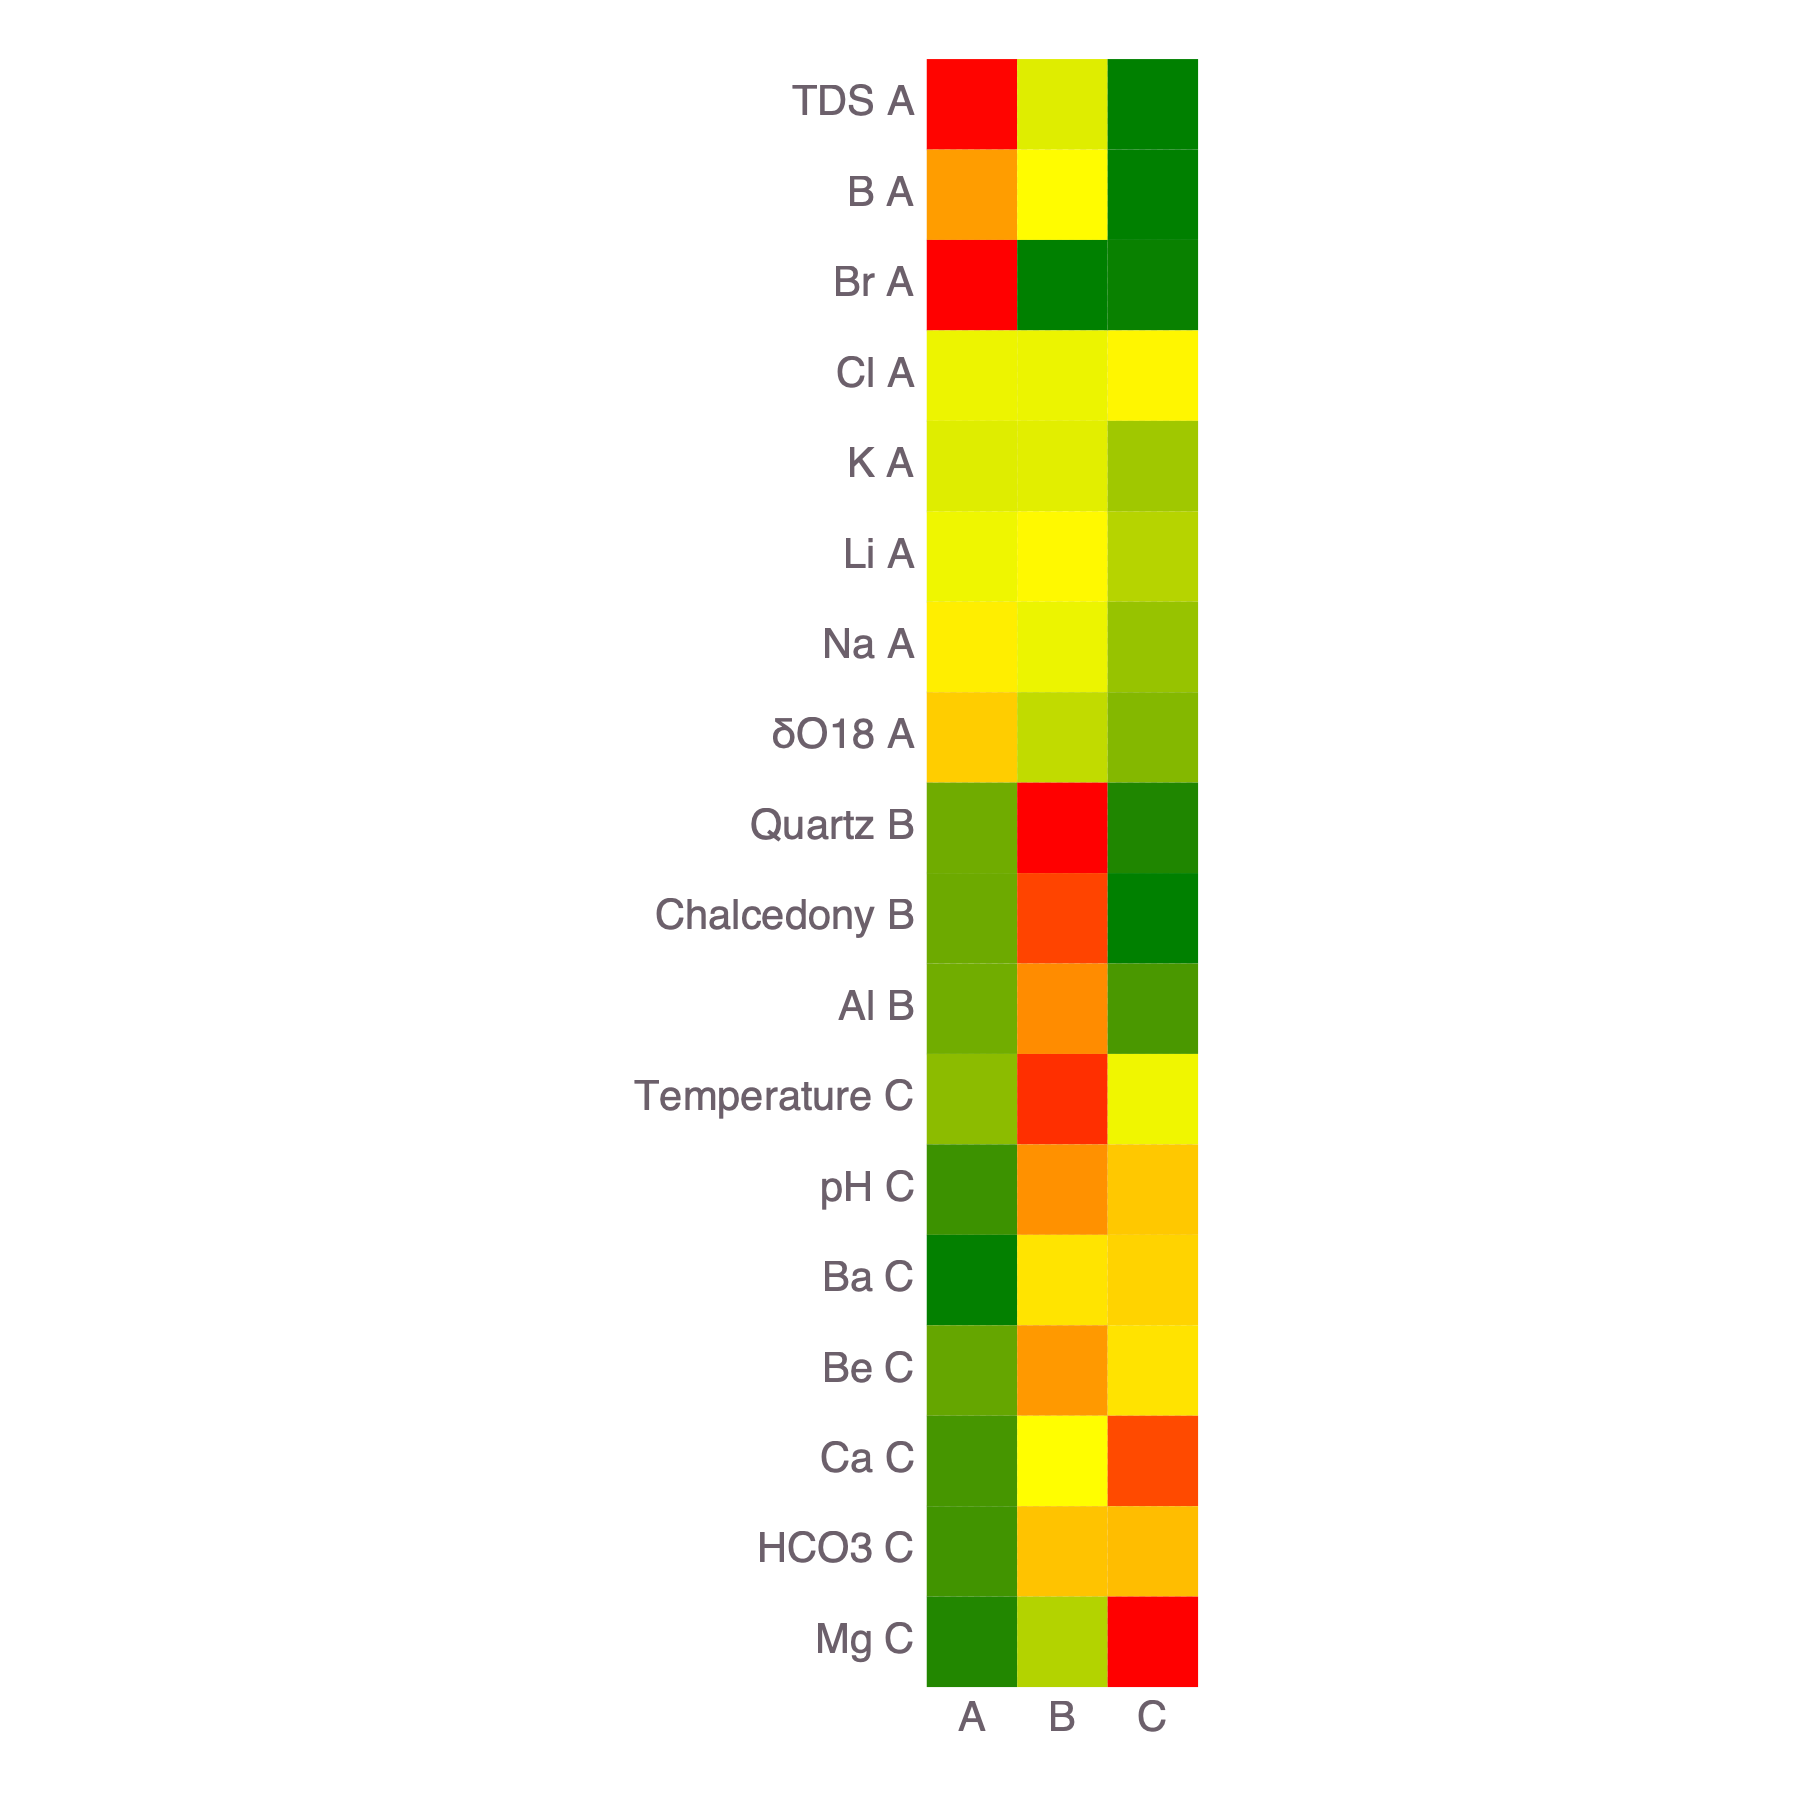
\includegraphics{../figures-postprocessing-nl-640/attributes-3-labeled-sorted.png}
\caption{attributes-3-labeled-sorted}
\end{figure}

The well locations are also clustered into \textbf{3} groups. The
grouping is based on analyses of the location matrix \texttt{H}.

A spatial map of the locations is obtained:

\begin{figure}
\centering
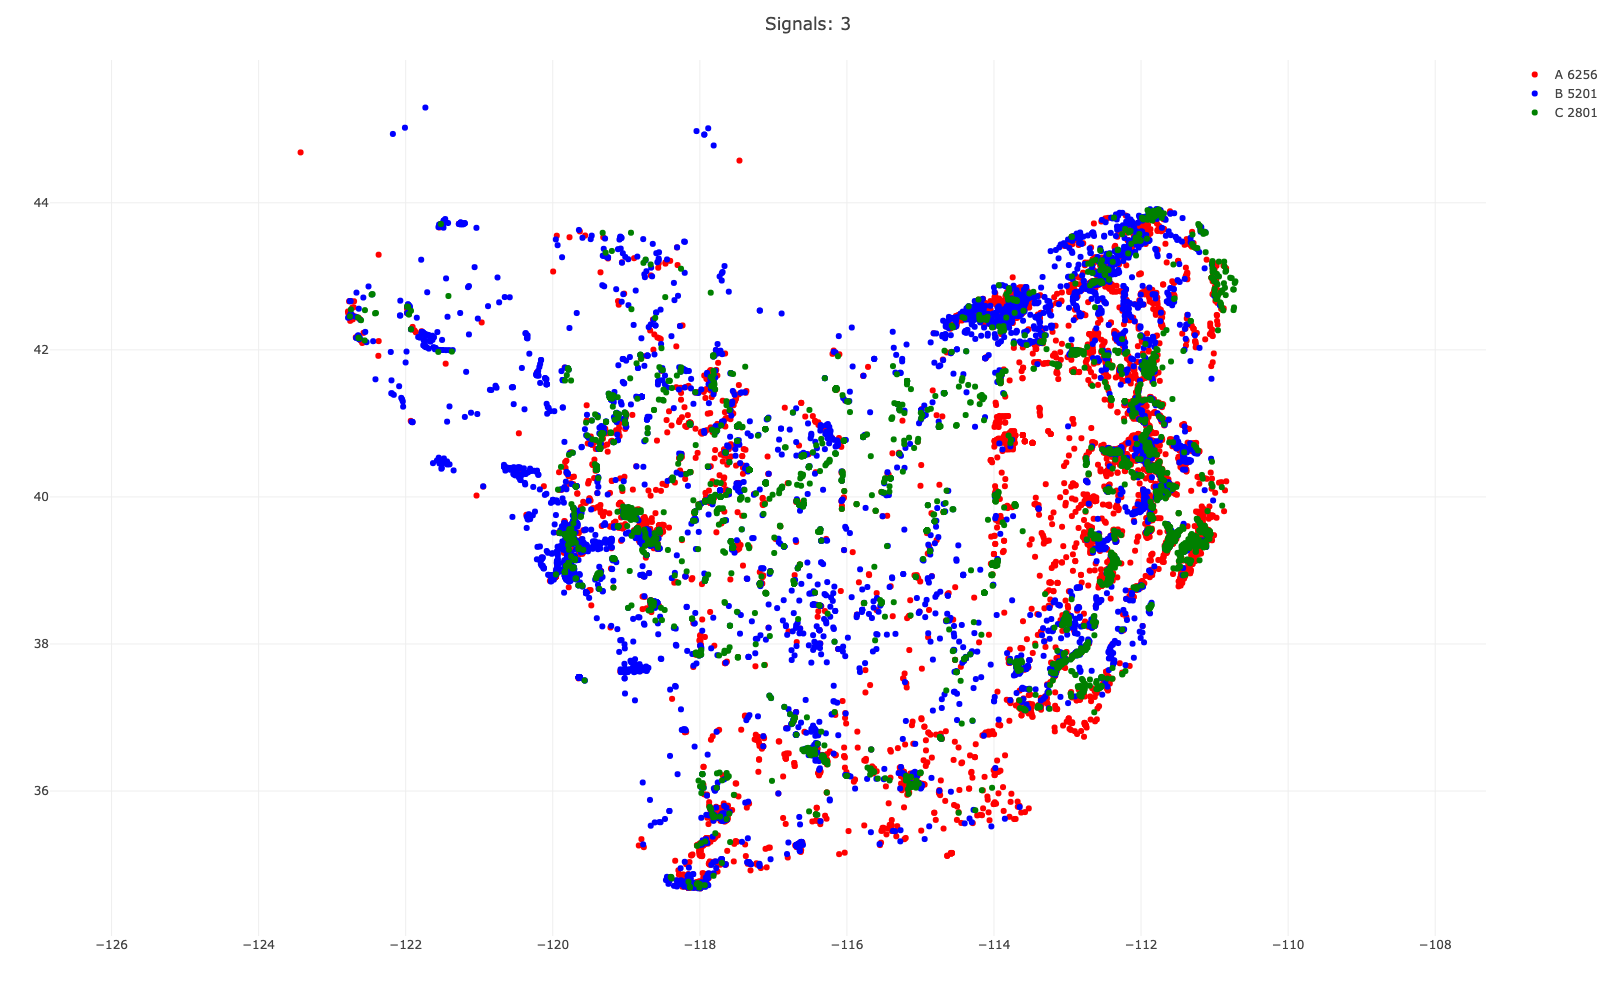
\includegraphics{../figures-postprocessing-nl-640/locations-3-map.png}
\caption{locations-3-map}
\end{figure}

The map \url{../figures-postprocessing-nl-640/locations-3-map.html}
provides interactive visualization of the extracted location groups (the
html file can be also openned with any browser).

\begin{verbatim}
<iframe src="../figures-postprocessing-nl-640/locations-3-map.html" frameborder="0" height="800" width="50%"></iframe>
\end{verbatim}

    \hypertarget{discussion-of-nmfk-results}{%
\subsubsection{Discussion of NMFk
results}\label{discussion-of-nmfk-results}}

Our ML algorithm extracted \textbf{3} signatures in the analyzed
dataset.

Signature \textbf{B} is detected at 5201 locations shown in the map
above.

At these locations, \texttt{Temperature}, \texttt{Quartz},
\texttt{Chalcedony} and \texttt{Al} appear to be elevated. There is
general correlations between \texttt{Temperature}, \texttt{Quartz},
\texttt{Chalcedony} and \texttt{Al} observations at these locations. All
these locations can be identified as geothermal resources with high
prospectivity.

Signature \textbf{C} is detected at 2801 locations shown in the map
above.

At these locations, \texttt{Temperature} is also elevated. However,
\texttt{Quartz}, \texttt{Chalcedony} and \texttt{Al} are low. However,
\texttt{Ca} and \texttt{Mg} are elevated as well. All these locations
can be identified as geothermal resources with lower prospectivity.
Additional analyses and data acquisition activities are needed to define
their prospectivity.

Signature \textbf{A} is detected at 6256 locations shown in the map
above.

At these locations, \texttt{TDS}, \texttt{B} and \texttt{Br} are
elevated. However, the \texttt{Temperature} is low. These locations can
be identified as geothermal resources with low prospectivity.

Biplots are also generated by the scripts presented above to map the
interelations between the attributes as defined by the extraced
\textbf{3} signatures which can be viewed also as basis vectors. The
interpretation of the biplots is consistent with the way eigen-analysis
(SVD/PCA) biplots are also interpreted.

\begin{figure}
\centering
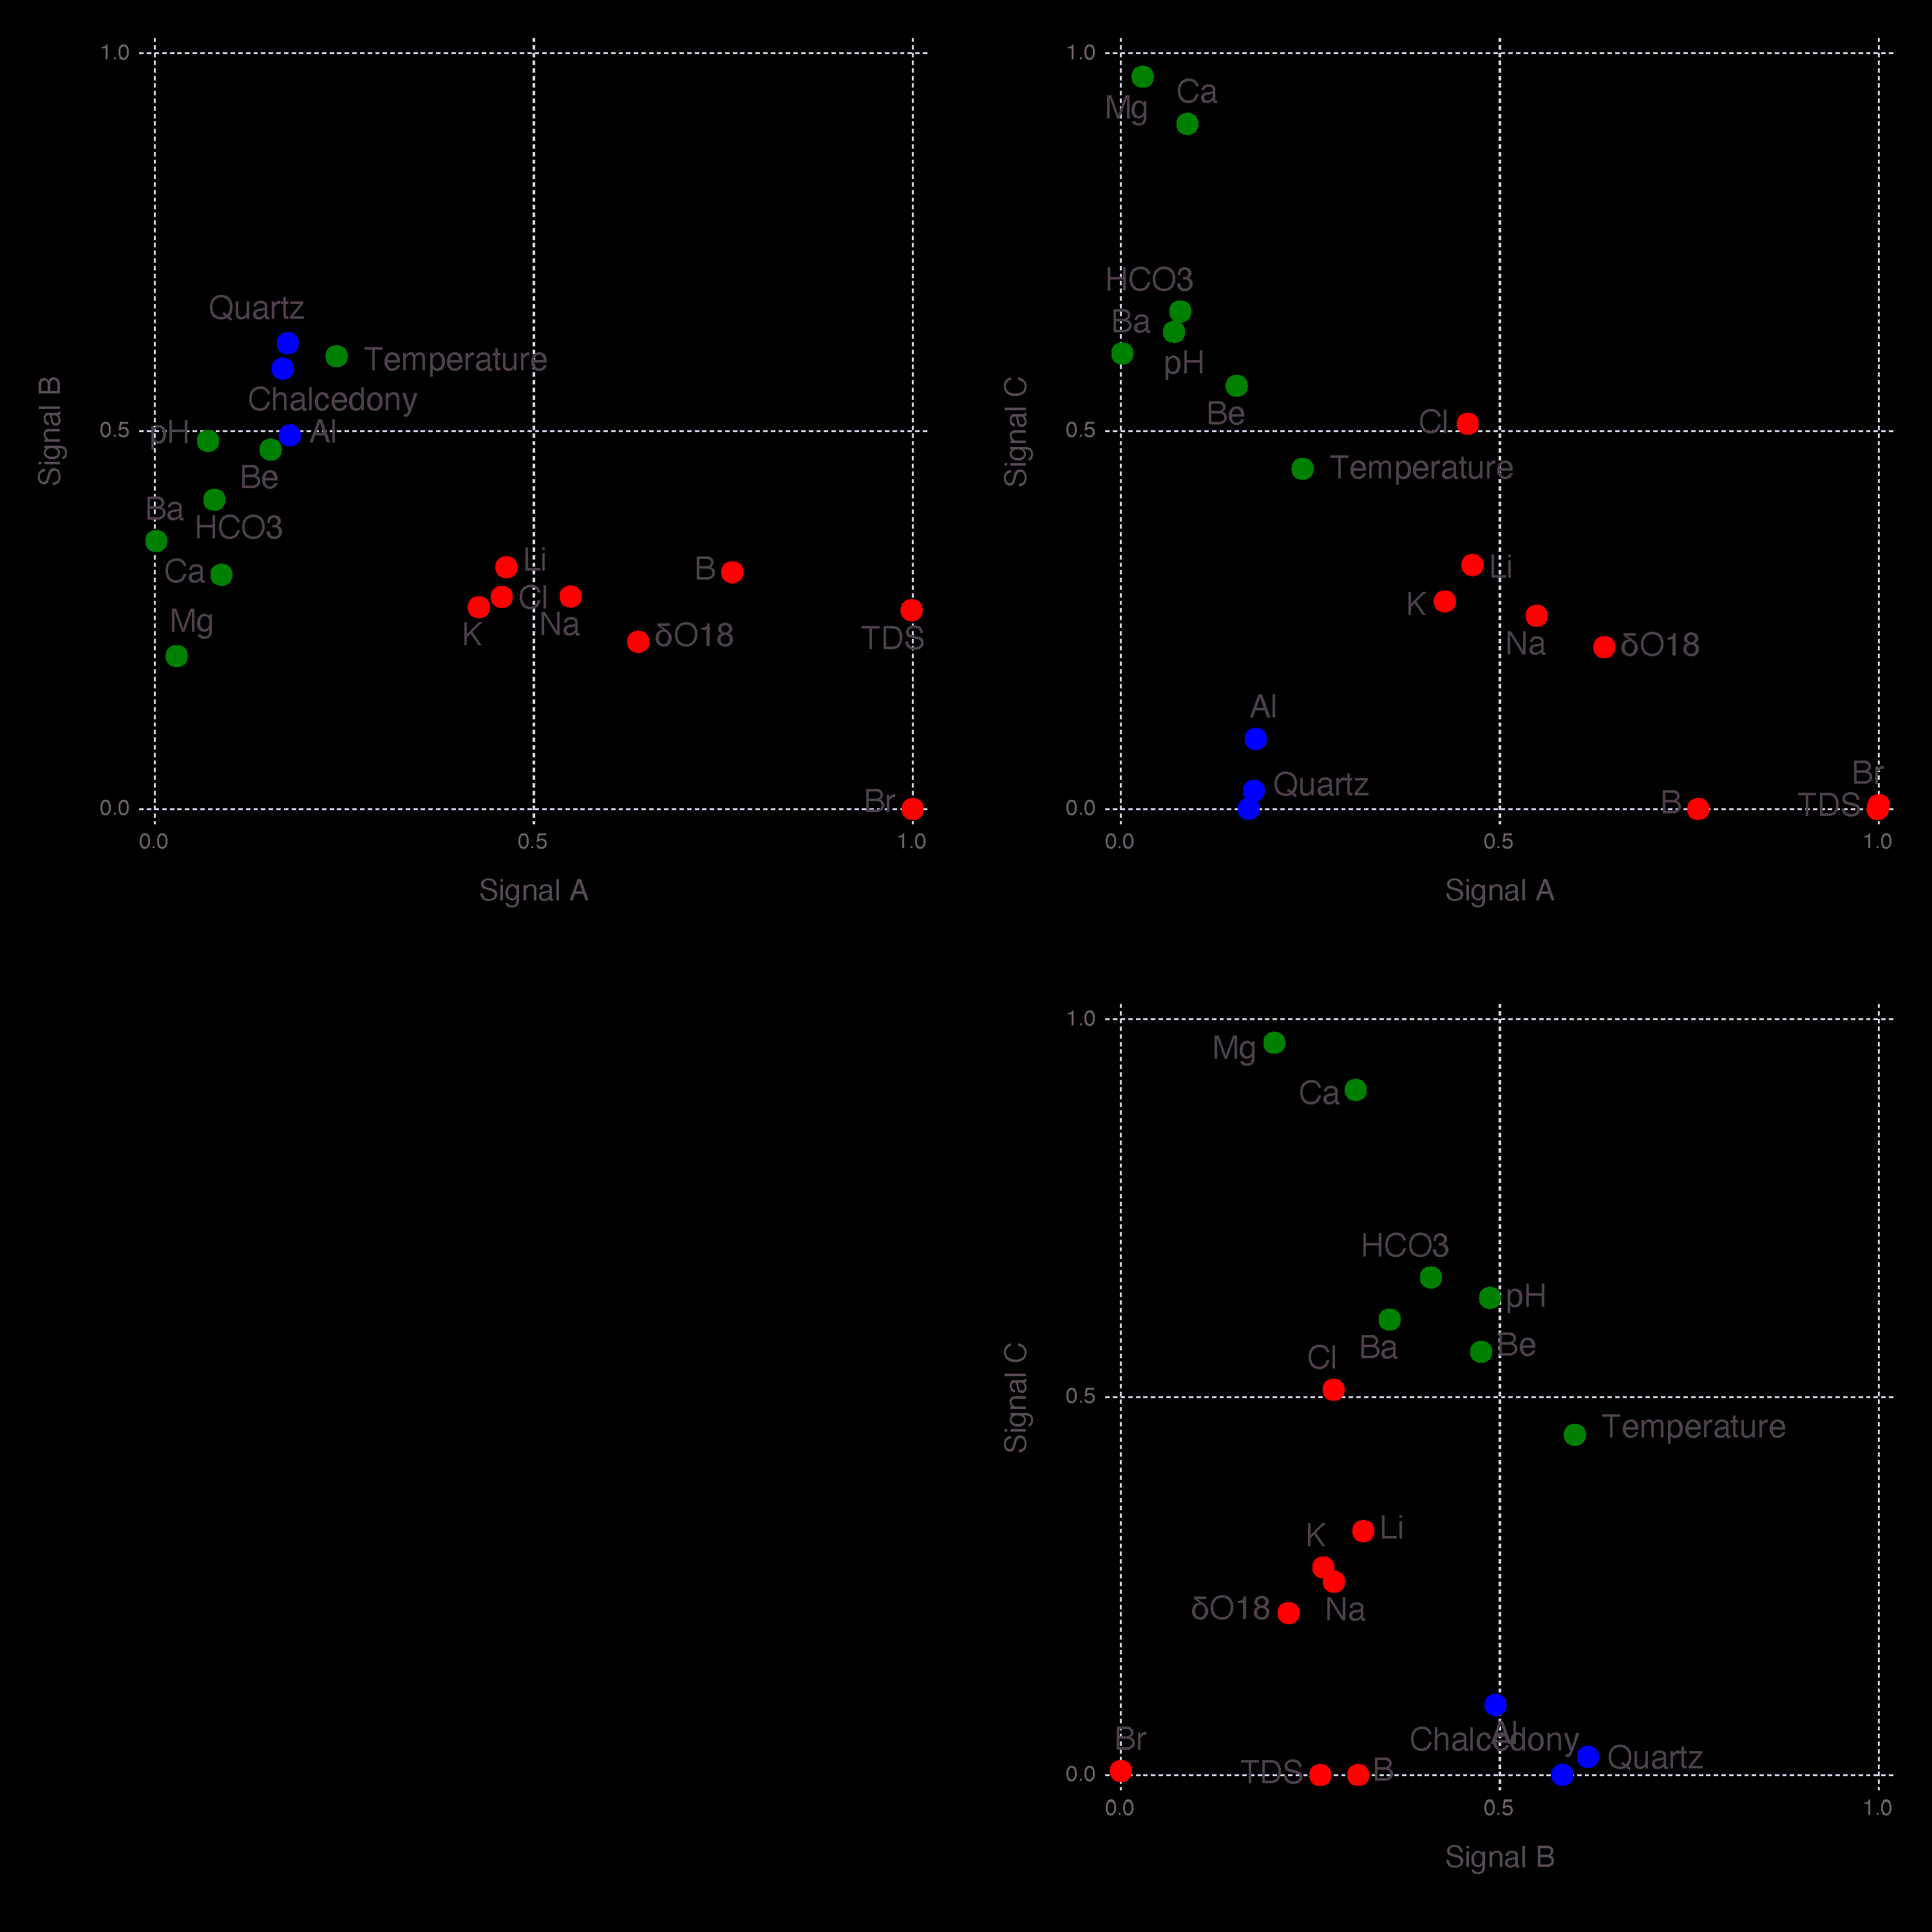
\includegraphics{../figures-postprocessing-nl-640/attributes-3-biplots-labeled.png}
\caption{attributes-3-biplots-labeled}
\end{figure}

It clear from the figure above, that \texttt{Temperature},
\texttt{Quartz}, \texttt{Chalcedony} and \texttt{Al} are generally
collocated.

\texttt{Ca} and \texttt{Mg} are also collocated.

Similarly, \texttt{K}, \texttt{Li} and \texttt{Na} are also collocated.

The coloring of the dots represents the ML clustering of the attributes
into \textbf{3} groups.

The figure demonstrates that ML algorithm successfully identified
attributes which have generally similar spatial patterns.

The biplots can also map the locations at which the data are collected
as shown in the figure below.

\begin{figure}
\centering
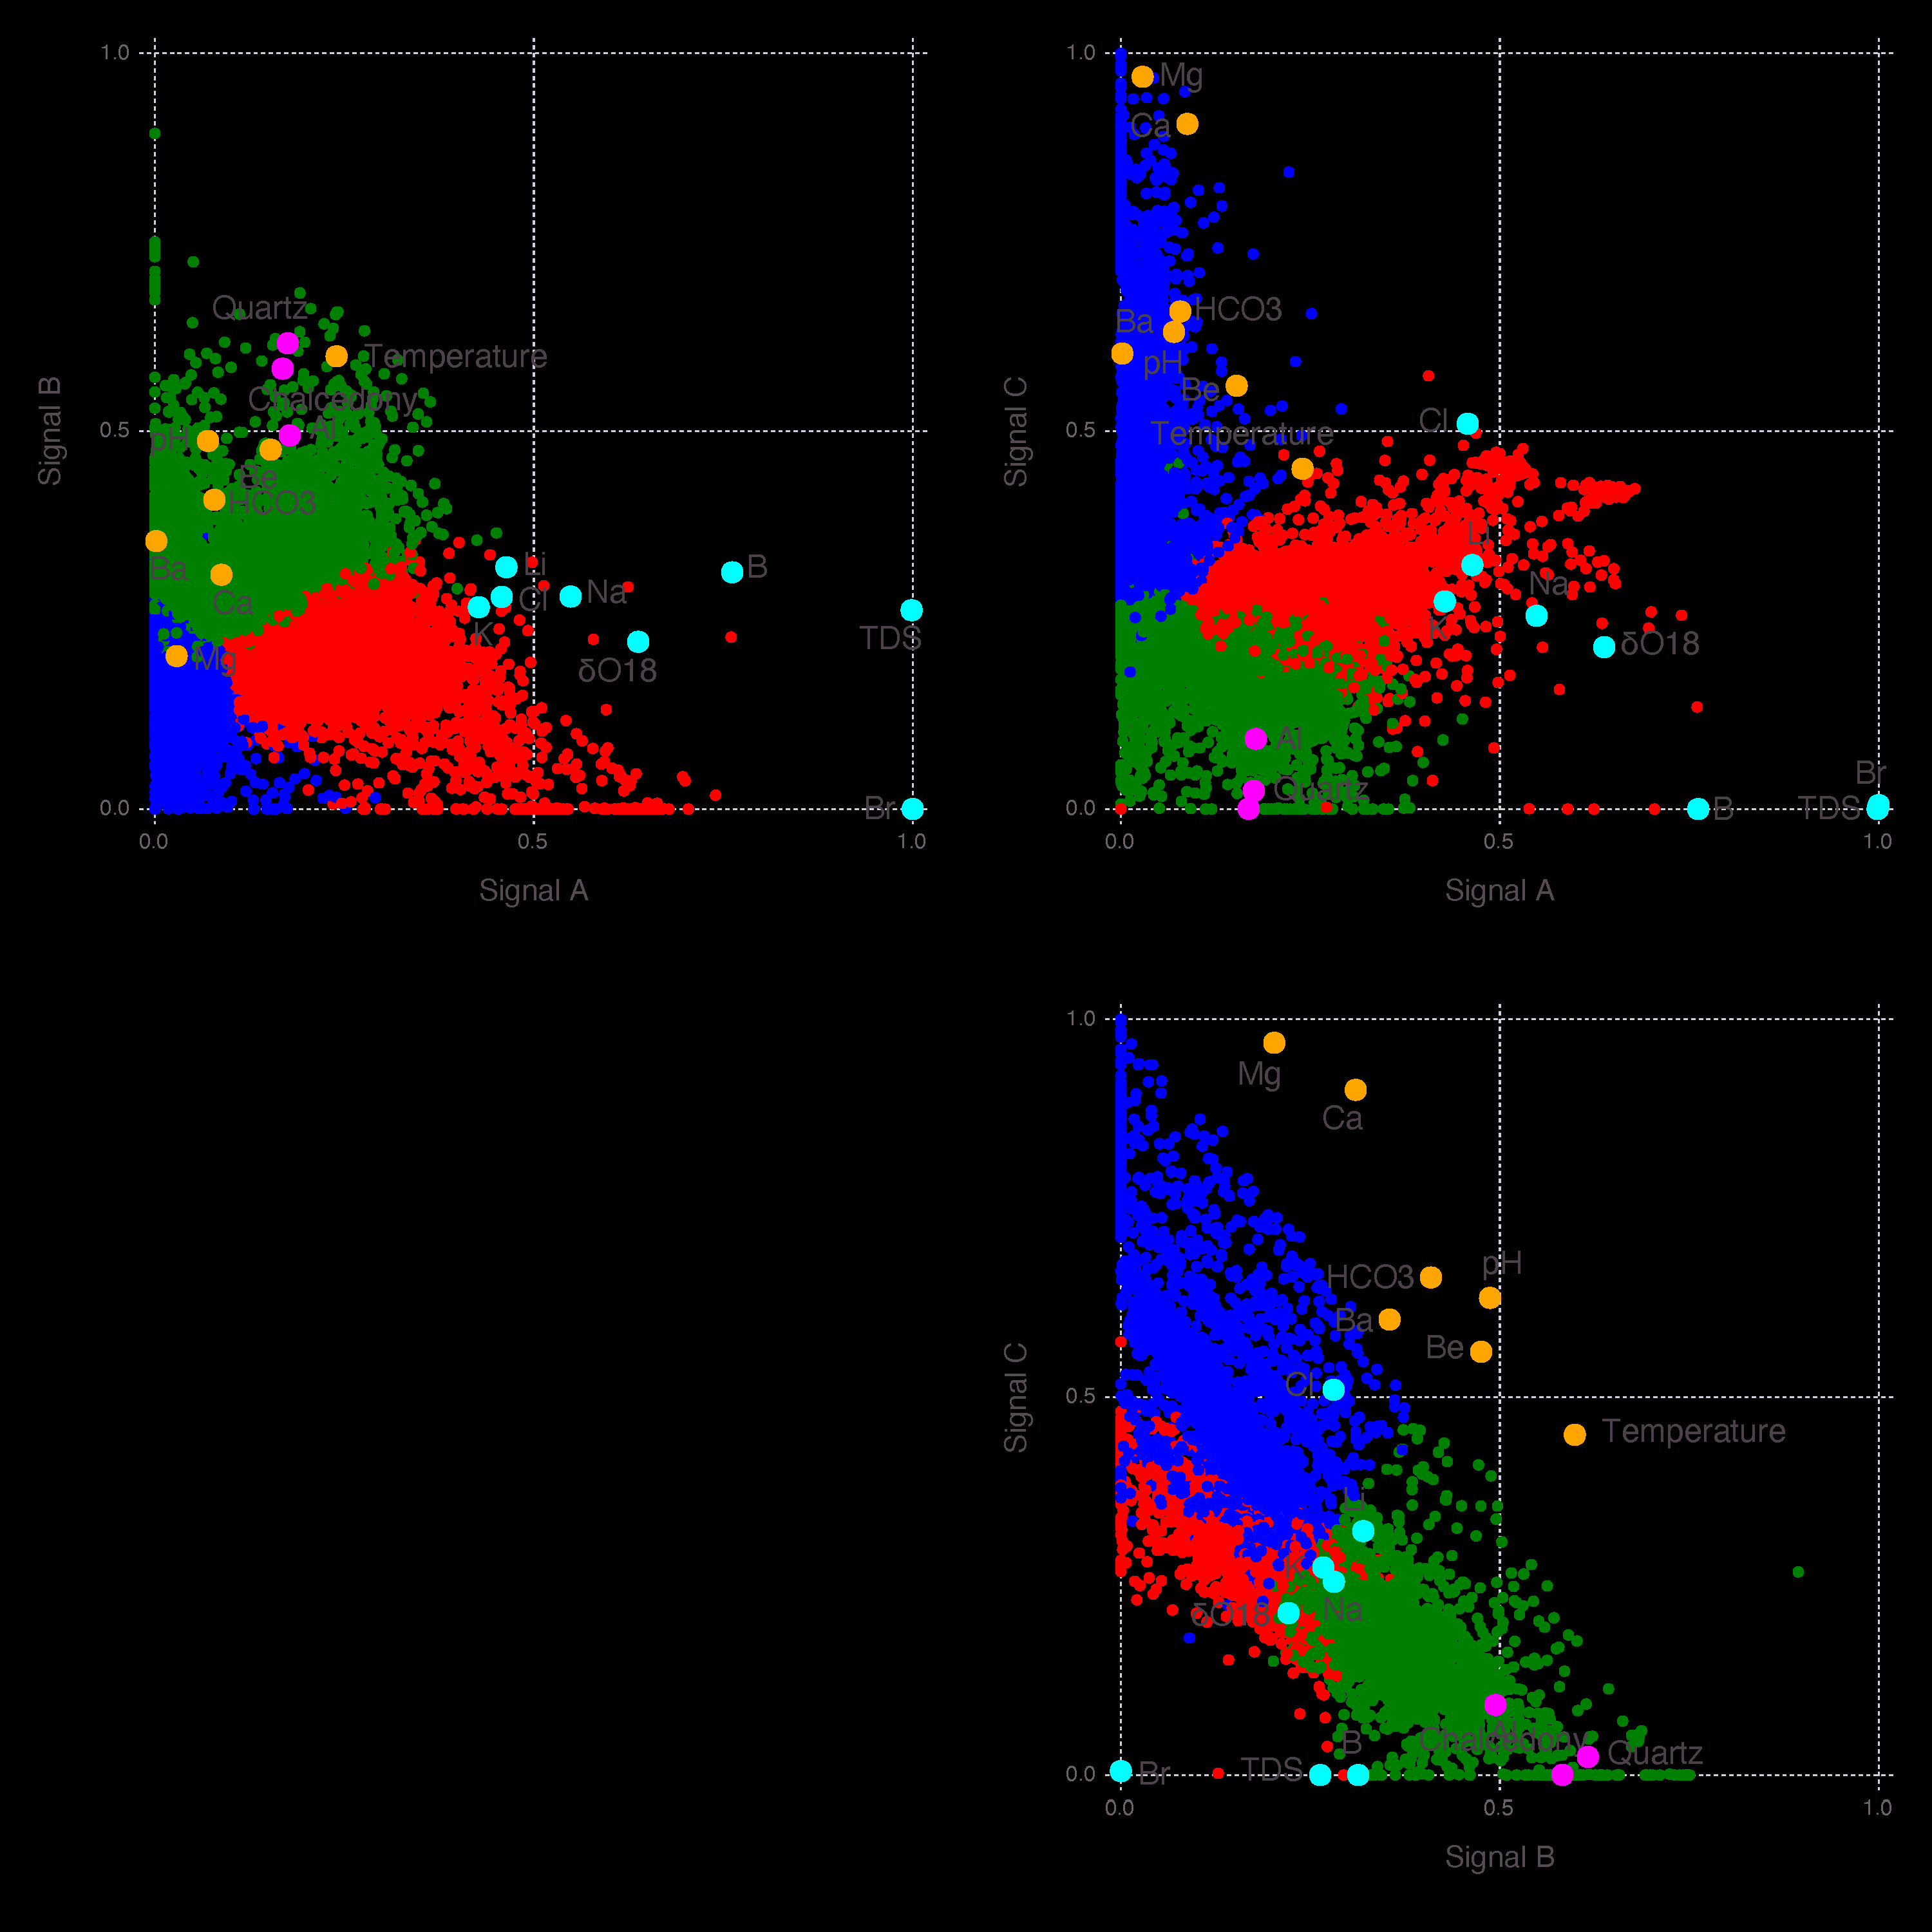
\includegraphics{../figures-postprocessing-nl-640/all-3-biplots-labeled.png}
\caption{all-3-biplots-labeled}
\end{figure}

The coloring of the dots represents the ML clustering of the attributes
and locations into \textbf{3} groups each (\textbf{6} groups in total).

The biplots above show how the attribute data is applied to label the
locations so that they are optimally grouped into \textbf{3} locations
clusters.


    % Add a bibliography block to the postdoc
    
    
    
\end{document}
